%% Master draft, journal version (IEEE Internet of Things Journal, double column).
%% The conference version is cut from this text.
\documentclass[journal]{IEEEtran}
\IEEEoverridecommandlockouts

\usepackage{cite}
\usepackage{amsmath,amssymb,amsfonts}
\let\proof\relax
\let\endproof\relax
\usepackage{amsthm}
\usepackage{algorithm}
\usepackage{algpseudocode}
\usepackage{graphicx}
\usepackage{booktabs}
\usepackage{xcolor}
\usepackage{tikz}
\usetikzlibrary{arrows.meta,positioning}

\newtheorem{assumption}{Assumption}
\newtheorem{definition}{Definition}
\newtheorem{lemma}{Lemma}
\newtheorem{proposition}{Proposition}
\newtheorem{corollary}{Corollary}
\newtheorem{theorem}{Theorem}
\theoremstyle{remark}
\newtheorem{remark}{Remark}
\newtheorem{example}{Example}

\newcommand{\E}{\mathbb{E}}
\newcommand{\Prob}{\mathbb{P}}
\newcommand{\ind}[1]{\mathbf{1}\{#1\}}
\newcommand{\A}{\mathcal{A}}
\newcommand{\I}{\mathcal{I}}
\newcommand{\lab}{\ell}
\newcommand{\Dbar}{\bar{\Delta}}
\newcommand{\ee}{\varepsilon}
\newcommand{\xh}{\hat{x}}

\begin{document}

\title{Speak When Sure, Ask When Unsure: Confidence-Aware Status Updates from On-Board Classifiers in Aerial IoT}

\author{Sameh~Hosny and John~Tadrous%
\thanks{S. Hosny is with the Akian College of Science and Engineering, American University of Armenia, Yerevan, Armenia (e-mail: \{email\}).}%
\thanks{J. Tadrous is with the Department of Electrical and Computer Engineering, Gonzaga University, Spokane, WA, USA (e-mail: tadrous@gonzaga.edu).}}

\maketitle

\begin{abstract}
Internet of Things (IoT) devices increasingly classify their sensor data on board and transmit a label of a few bytes instead of the raw data. A small on-board classifier errs, however, and a wrong label misleads the receiver. We study an unmanned aerial vehicle (UAV) that monitors a scene for a ground station (GS) and, in every slot, stays silent, sends its on-board label, or uploads the raw frame to a more accurate ground classifier. The goal is to minimize the long-run average age of incorrect information (AoII) of the GS status under an average energy budget and an intermittent air-to-ground link. The UAV never observes the true state, so we formulate a constrained partially observable Markov decision process and show that a belief over the current AoII is a sufficient statistic. The belief is updated with the calibrated confidence of each frame, divided by the class prior and tempered to account for errors that are correlated in time. From this belief we derive the one-step expected AoII of each action in closed form, prove that a label that agrees with the GS status is never worth sending, and show that the drift-plus-penalty rule reduces to confidence thresholds ordered silent, raw, label. The resulting policy, CA-DPP, meets the energy budget on every sample path and stores its belief in about 1.2\,kB. We evaluate it on Sentinel-2 flood-mapping traces with five-fold cross-validation over image chips and paired tests over 20 held-out runs. For budgets up to 2\,mJ per slot it lowers the average AoII by 52\% to 75\% relative to pre-identification and age-threshold policies ($p<10^{-5}$). Relative to an AoII-threshold policy, it lowers the AoII by $22\%\pm12\%$ at 0.25\,mJ per slot ($p=0.002$) and, at 0.5\,mJ per slot, by 27\% and 49\% when the on-board accuracy falls to 84\% and 82\% ($p<10^{-5}$). With an accurate classifier and ample energy the two policies are statistically indistinguishable.
\end{abstract}

\begin{IEEEkeywords}
Age of incorrect information, on-board inference, aerial IoT, UAV, Lyapunov optimization, POMDP, calibration.
\end{IEEEkeywords}

%% =====================================================================
\section{Introduction}\label{sec:intro}
%% =====================================================================
\IEEEPARstart{M}{any} Internet of Things (IoT) devices no longer send what they sense. A camera trap reports that it saw an animal, a nanosatellite reports that a pixel block contains a ship, and an unmanned aerial vehicle (UAV) that surveys a flood reports that the area below it is under water. Each of these devices runs a small classifier on board and transmits its decision, a label of a few bytes, instead of an image of tens of kilobytes~\cite{shamsoshoara2021flame,kyrkou2020aider,hosny2026tinysem}. For a battery-powered device on a weak wireless link, this saves most of the energy and airtime that a raw upload would cost.

The saving comes at a price. A classifier small enough to run on a UAV or a microcontroller makes mistakes, and it makes them most often on ambiguous inputs: a flooded field under cloud shadow, a dry field after rain. Once the transmitted content is an inference, a delivered update can be wrong. The receiver then holds a fresh but wrong estimate, and it keeps it until a later update corrects it. The age of information (AoI) does not register this error, because it resets on every delivery whether the content is right or wrong. The age of incorrect information (AoII)~\cite{maatouk2020aoii} grows while the receiver's estimate differs from the true state, so it penalizes wrong estimates as well as stale ones. It is the natural measure of how well the receiver knows the scene.

Existing AoII work assumes, however, that the transmitter observes the source through a sensor~\cite{maatouk2020aoii,zakeri2023aoiieh,ngo2025eh}. Such a transmitter knows whether the receiver is wrong and can decide to update exactly when it is. A device whose sensor is a classifier has no such knowledge. It sees only its own label and how confident the classifier is about it. A confident label that disagrees with the receiver probably means that the receiver is wrong. An unsure label could mean either, and sending it may turn a correct estimate into a wrong one. The device has a third option: it can upload the raw data and let a larger classifier on the ground decide, at a much higher energy cost that depends on the link.

Consider a UAV that maps a flood for a ground station (GS) that coordinates rescue teams. If a frame looks clearly flooded and the GS status says dry, the UAV should send its label. If the frame is ambiguous, it should upload the frame when the link is good enough, and wait otherwise. If its label agrees with the GS status, it should stay silent. This paper turns these rules of thumb into a policy with guarantees. Four difficulties stand in the way. First, the UAV never observes whether the GS is wrong. Second, the confidence of a small classifier is itself noisy, and its errors are correlated across consecutive frames because consecutive footprints overlap. Third, the delivery probability and energy of each action depend on the distance to the GS and on blockage. Fourth, the UAV has a fixed energy budget for the whole mission, so a transmission now reduces what is available later.

The UAV keeps a belief over the current AoII of the GS status, updated with the calibrated confidence of each frame and with the acknowledgments of the GS. From the belief we compute in closed form how much each action reduces the expected AoII of the next slot, and a Lyapunov drift-plus-penalty rule weighs this reduction against the energy cost, with a price that rises when the UAV overspends. The main contributions are as follows.
\begin{enumerate}
\item \emph{Model.} We formulate confidence-aware status updating as a constrained partially observable Markov decision process (POMDP). It couples a calibrated per-sample error model of the on-board classifier, a ground classifier, an intermittent air-to-ground link and an energy budget. We show that a belief over the current AoII is a sufficient statistic, and we derive its update, including a prior correction and a tempered likelihood for errors that are correlated in time (Sections~\ref{sec:model} and~\ref{sec:belief}).
\item \emph{Structure.} We derive the one-step expected AoII of each action in closed form. We prove that a label that agrees with the GS has no value and that the per-slot decision has a threshold structure in the confidence: the UAV stays silent at low confidence, uploads the raw frame at intermediate confidence, and sends the label at high confidence (Section~\ref{sec:structure}).
\item \emph{Policy.} We build the online policy CA-DPP on these results and prove that it meets the energy budget on every sample path. CA-DPP needs no knowledge of the confidence distribution, the blockage statistics or the trajectory, and its per-slot cost is linear in the size of the belief (Section~\ref{sec:lyap}).
\item \emph{Evaluation.} We evaluate CA-DPP on inference traces from the Sen1Floods11 dataset~\cite{bonafilia2020sen1floods11} under chip-level cross-validation, against policies adapted from four recent designs~\cite{zakeri2023aoiieh,gan2025taoi,pehlivanoglu2026orbit,basnayaka2025aomi}. We identify when the per-frame confidence pays off: under tight energy budgets and with weak on-board classifiers. We also identify when it does not: with an accurate classifier and ample energy, simpler policies perform as well (Sections~\ref{sec:results} and~\ref{sec:discussion}).
\end{enumerate}

The rest of the paper is organized as follows. Section~\ref{sec:related} reviews related work. Section~\ref{sec:model} presents the system model. Section~\ref{sec:problem} formulates the problem and derives the belief of the UAV about the AoII. Section~\ref{sec:structure} derives the value of each action and the structure of the per-slot decision. Section~\ref{sec:lyap} presents CA-DPP and its energy guarantee. Section~\ref{sec:results} reports the evaluation, Section~\ref{sec:discussion} discusses its implications and limitations, and Section~\ref{sec:concl} concludes. The proofs are in the appendix.

%% =====================================================================
\section{Related Work}\label{sec:related}
%% =====================================================================
This work draws on three lines of research: AoII and its optimization, freshness metrics for systems in which the transmitted content is an inference, and the offloading of inference from IoT devices and UAVs. We review each line and then summarize how our work differs.

\subsection{Age of Incorrect Information}
The AoI measures the time since the latest received update was generated. It treats every update as correct, so it cannot tell a receiver with a fresh wrong estimate from one with a fresh correct estimate. Maatouk et al.~\cite{maatouk2020aoii} introduced the AoII to fix this. The AoII is zero while the receiver's estimate equals the source state and grows with time while the two differ. For a Markov source observed perfectly by the transmitter, they showed that the optimal policy transmits only when the estimate is wrong.

Two recent works add energy constraints. Zakeri et al.~\cite{zakeri2023aoiieh} study an energy-harvesting sensor that decides when to sample and when to transmit. Since the sensor does not see the source between samples, they formulate a POMDP whose belief is about the source state, and they derive threshold policies on the AoII. Ngo et al.~\cite{ngo2025eh} study the age and the correctness of updates from many energy-harvesting devices that share a random-access channel. In both works, a sample reveals the source state without error. Our UAV, in contrast, never observes the state. Its only observation is a classifier output that may be wrong, and the probability that it is wrong changes from frame to frame.

\subsection{Freshness of Inferred Information}
Several works consider status updates whose content is the output of a classifier. Buratto et al.~\cite{buratto2023misclass} add a penalty for misclassification to an AoI scheduling problem. The classifier errs with a fixed probability, and the schedule is computed offline. Gan et al.~\cite{gan2025taoi} define a task-oriented AoI for cameras that pre-identify each frame on the device and send the frames that appear to contain the target to a server, which re-identifies them with a larger model. The error rates of both classifiers are fixed, so the device does not use the confidence of individual frames. Pehlivano\u{g}lu, Li and Uysal~\cite{pehlivanoglu2026orbit} let a satellite choose among idling, running inference on board, sending a cached result and offloading raw data to the ground. Their action set is the closest to ours. They prove that a threshold policy minimizes the age of inference, but each action succeeds with a fixed probability, errors do not depend on the sample, and energy is not constrained. Basnayaka et al.~\cite{basnayaka2025aomi} define the age of misclassified information for event detection from low Earth orbit, again with a constant classification accuracy.

These works establish that the correctness of an inferred update matters for freshness. All of them, however, describe the classifier by a single error rate. A calibrated classifier gives more information than that: it reports, for each frame, how likely its label is to be wrong. We show how to use this information in the decision to stay silent, send a label or ask the ground.

\subsection{Inference Offloading from IoT Devices and UAVs}
A large body of work decides whether an IoT device or a UAV should run a task locally or offload it to an edge server, usually to minimize delay or energy. Yang et al.~\cite{yang2020uav}, for example, jointly optimize the offloading decisions and the trajectory of a UAV under energy constraints. Our Tiny-SEM framework~\cite{hosny2026tinysem} models the noise of a small semantic encoder and manages the energy of the device with a queue. These works model classifier noise and energy, but they do not measure how fresh or how correct the receiver's knowledge is. Datasets such as FLAME~\cite{shamsoshoara2021flame} for wildfires and AIDER~\cite{kyrkou2020aider} for disaster scenes show that classifiers small enough for a UAV reach useful accuracy, but they also show that such classifiers err on a noticeable fraction of the frames. Post-hoc calibration~\cite{guo2017calibration} makes the output score of such a classifier a reliable probability, which is what our belief update requires.

The energy constraint in our problem is handled with Lyapunov drift-plus-penalty~\cite{neely2010book}. Huang and Neely~\cite{huang2013eh} extend this method to devices that harvest energy into a finite battery. Since the AoII depends on past decisions, the standard performance bound of drift-plus-penalty does not apply directly. The renewal framework of~\cite{neely2013renewal} is the natural tool for such problems, and we discuss it in Section~\ref{sec:lyap}.

\subsection{Positioning}
Table~\ref{tab:positioning} compares the closest works on four elements: (E1) a per-sample error model driven by the classifier confidence; (E2) AoII on the inferred label; (E3) an energy constraint handled online; and (E4) a choice among silence, a label and raw data. Each prior work covers at most two of these elements fully. Ours combines all four.

\begin{table}[t]
\caption{Positioning against the closest works. \checkmark: covered; $\circ$: partly covered; --: not covered.}
\label{tab:positioning}
\centering\footnotesize
\setlength{\tabcolsep}{3pt}
\resizebox{\columnwidth}{!}{%
\begin{tabular}{@{}lcccc@{}}
\toprule
Work & (E1) per-sample & (E2) AoII on & (E3) online & (E4) silent/\\
 & errors & inferred label & energy & label/raw\\
\midrule
Zakeri et al.~\cite{zakeri2023aoiieh} & -- & \checkmark & $\circ$ & $\circ$\\
Ngo et al.~\cite{ngo2025eh} & -- & $\circ$ & $\circ$ & --\\
Buratto et al.~\cite{buratto2023misclass} & $\circ$ & \checkmark & -- & --\\
Gan et al.~\cite{gan2025taoi} & $\circ$ & $\circ$ & -- & $\circ$\\
Pehlivano\u{g}lu et al.~\cite{pehlivanoglu2026orbit} & -- & $\circ$ & -- & \checkmark\\
Basnayaka et al.~\cite{basnayaka2025aomi} & $\circ$ & $\circ$ & -- & --\\
Yang et al.~\cite{yang2020uav} & $\circ$ & -- & $\circ$ & $\circ$\\
\midrule
This work & \checkmark & \checkmark & \checkmark & \checkmark\\
\bottomrule
\end{tabular}}
\end{table}

%% =====================================================================
\section{System Model}\label{sec:model}
%% =====================================================================
\subsection{Network and Scenario}\label{sec:story}
We consider a UAV that flies over a disaster area and reports to a ground station (GS) that coordinates the response, as shown in Fig.~\ref{fig:system}. Time is divided into slots of length $\tau$, indexed by $t\in\{0,1,\dots\}$. The UAV flies at constant speed along a route planned before the mission, so its position $\mathbf{u}(t)$ in every slot is known in advance. In each slot the UAV photographs the patch of ground below it, which we call its footprint, and a small classifier on board decides whether an event of interest is present in the patch, for example flooding, fire, a collapsed building or a survivor. Throughout the paper we use flood mapping as the running example: the classifier labels each photo ``flooded'' or ``dry'', and the response teams need to know which patches are under water. The model applies to any such event with a suitable classifier.

Since the UAV moves, the patch below it changes from slot to slot, and consecutive footprints partly overlap. We do not model the whole area. We model only what the UAV sees along its route: in slot $t$, $X(t)$ is the state of the patch below the UAV and $Y(t)$ is the photo of that patch. The position $\mathbf{u}(t)$ affects the model in one place only, the link to the GS. The distance and the elevation angle to the GS determine how likely a packet is to arrive and how much energy it costs. The route can have any shape. In our evaluation it is a circle, so the UAV passes alternately through parts of the route close to the GS and far from it.

The GS has no sensor of its own. Everything it knows about the patch below the UAV comes from the UAV. We call the GS status the label that the GS currently holds for this patch: it is the last label the GS received, either a label sent by the UAV or the label that a larger classifier at the GS produced from a photo sent by the UAV. The GS holds this status until the next update arrives, and the response teams act on it. In each slot the UAV can therefore stay silent, send its on-board label, or send the photo. A label is a few bytes and cheap to send, but it may be wrong. A photo is tens of kilobytes and much more expensive, and it may fail to arrive far from the GS, but the ground classifier labels it almost always correctly. The UAV chooses under an energy budget and without observing the true state. Table~\ref{tab:notation} summarizes the notation.

\begin{figure}[t]
\centering
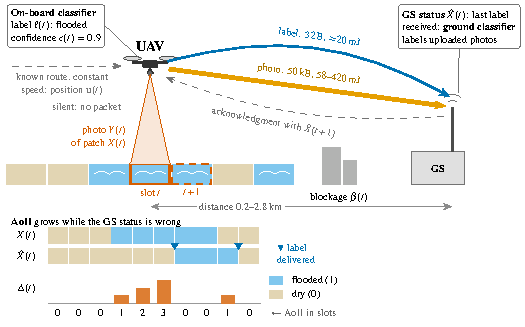
\includegraphics[width=\columnwidth]{figures/fig_scenario.pdf}
\caption{The scenario. A UAV flies over a disaster area (flooding in this example), photographs the patch below it and labels the photo on board with a confidence. In each slot it stays silent, sends its label (blue), or sends the photo to the ground classifier (orange). The GS status is the last label received, and every packet is acknowledged with it. Buildings can block the link, and the cost of a photo grows with the distance. Inset: the AoII grows by one per slot while the GS status is wrong and returns to zero when a delivered label or a change of the scene makes it right.}
\label{fig:system}
\end{figure}

\begin{table}[t]
\caption{Main notation}\label{tab:notation}
\centering\footnotesize
\setlength{\tabcolsep}{3pt}
\begin{tabular}{@{}p{0.52\columnwidth}ll@{}}
\toprule
Meaning & Symbol & Defined in\\
\midrule
Patch below the UAV: event or not & $X(t)$ & \eqref{eq:source}\\
How often the scene changes & $p_0,p_1$; $\varpi$ & \eqref{eq:source}, \eqref{eq:stationary}\\
Photo; on-board label, confidence & $Y(t)$; $\lab(t)$, $c(t)$ & \eqref{eq:calib}\\
Label disagrees with the GS status & $d(t)$ & Sec.~\ref{sec:belief}\\
Label from the ground classifier & $\lab^{\rm g}(t)$, $\ee_{\rm g}(c)$ & Assum.~\ref{as:inf}\\
Silent, send label, send photo & $a(t)\in\{0,1,2\}$ & Sec.~\ref{sec:act}\\
UAV position, blockage & $g(t)$ & \eqref{eq:block}, \eqref{eq:pl}\\
Packet decoded & $o(t)$ & \eqref{eq:est}\\
Delivery probability; energy & $q_a(g)$; $E_a(g)$ & \eqref{eq:succ}, \eqref{eq:energy}\\
Energy budget of the mission & $\bar E$ & \eqref{eq:budget}\\
What the GS status says & $\hat X(t)$ & \eqref{eq:est}\\
How long the GS status has been wrong & $\Delta(t)$ (AoII) & \eqref{eq:aoii}\\
What the UAV believes about $\Delta(t)$ & $\pi_t$; $\mu_t$, $S_t$ & \eqref{eq:belief}, \eqref{eq:musum}\\
Evidence of a frame that the GS is wrong & $\Lambda_t$ & \eqref{eq:Lambda}\\
Value of an action; its energy price & $G_a$; $Z(t)$, $V$ & Secs.~\ref{sec:structure}, \ref{sec:lyap}\\
\bottomrule
\end{tabular}
\end{table}

\subsection{Event Dynamics}\label{sec:src}
\begin{figure}[t]
\centering
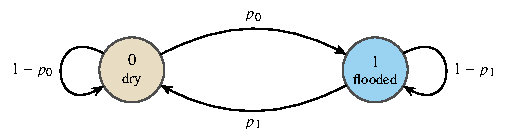
\includegraphics[width=0.7\columnwidth]{figures/fig_markov.pdf}
\caption{Markov chain of the patch state $X(t)$. In each slot a dry patch ($0$) is followed by a flooded one with probability $p_0$, and a flooded patch ($1$) by a dry one with probability $p_1$. On our flood data $p_0=0.039$ and $p_1=0.166$.}
\label{fig:markov}
\end{figure}
We describe the patch below the UAV by a binary state $X(t)\in\{0,1\}$, with $X(t)=1$ if the event is present and $X(t)=0$ otherwise. In the flood example, $X(t)=1$ means that the patch is flooded. The UAV moves a short distance between slots, so consecutive frames cover overlapping areas and the state tends to persist: a flooded footprint is usually followed by another flooded footprint. Note that $X(t)$ refers to the patch below the UAV in slot $t$, not to a fixed patch. The chain therefore describes how the state changes from one footprint to the next along the route, and its transition probabilities depend on the speed of the UAV and on the overlap of its footprints. They are constant because the speed is. The simplest model that captures this persistence is the two-state Markov chain of Fig.~\ref{fig:markov}. Let $p_x$ be the probability that the state leaves $x$ in one slot,
\begin{equation}\label{eq:source}
\Prob\big\{X(t+1)\neq x\mid X(t)=x\big\}=p_x,\qquad x\in\{0,1\}.
\end{equation}
We assume $0<p_0,p_1<\tfrac12$. The lower bound makes the chain irreducible, so the scene does change and every state is visited. The upper bound says that the state is more likely to stay than to change in one slot. This persistence is what makes an old status useful at all: if the state changed more often than not, the GS would do better by inverting its last label than by keeping it. We use the bound $p_x<\frac12$ in Section~\ref{sec:structure}.

The fraction of time the chain spends in each state follows from the balance between the two transitions. In steady state the probability flow from 0 to 1 equals the flow from 1 to 0, so $\varpi_0p_0=\varpi_1p_1$, and with $\varpi_0+\varpi_1=1$,
\begin{equation}\label{eq:stationary}
\varpi_1=\frac{p_0}{p_0+p_1},\qquad \varpi_0=\frac{p_1}{p_0+p_1}.
\end{equation}
We call $\varpi=(\varpi_0,\varpi_1)$ the class prior. The chain may be asymmetric. In our flood data a flooded footprint turns dry more often than a dry one floods ($p_0=0.039$, $p_1=0.166$), so only $\varpi_1=19\%$ of the footprints are flooded. We use the symmetric case $p_0=p_1$ only to state some results in a simpler form.

\subsection{On-Board and Ground Classification}
In slot $t$ the UAV takes a photo $Y(t)$ of the patch below it, which we also call a frame. The photo is used only to classify the patch; the UAV knows its position from the route and does not infer it from the photo. The on-board classifier returns a label and a confidence,
\begin{equation}\label{eq:label}
\lab(t)\in\{0,1\},\qquad c(t)\in[\tfrac12,1],
\end{equation}
where $\lab(t)$ is the state that the classifier finds more likely and $c(t)$ is the probability it assigns to that state. A classifier that outputs a probability $p$ of flooding, as most do, gives $\lab(t)=\ind{p\ge\frac12}$ and $c(t)=\max\{p,1-p\}$. The confidence is useful only if it means what it says. We therefore require that the classifier be calibrated: among all frames that receive label $\lab$ and confidence $c$, a fraction $c$ is truly in state $\lab$, for both label values,
\begin{equation}\label{eq:calib}
\Prob\big\{X(t)=\lab(t)\mid\lab(t),\,c(t)\big\}=c(t).
\end{equation}
Averaging~\eqref{eq:calib} over the two label values shows that a label with confidence $c$ is wrong with probability $1-c$. The converse does not hold. A classifier can have this property while being overconfident when it says ``flooded'' and underconfident when it says ``dry''. We need~\eqref{eq:calib} for each label value because the belief update below uses the probability of each state given the label, and flooded and dry patches are not equally common.

Modern classifiers are often overconfident, so~\eqref{eq:calib} does not hold out of the box. Post-hoc calibration~\cite{guo2017calibration}, such as isotonic regression on held-out data, restores it to a good approximation. Fig.~\ref{fig:inference}(a) shows that our on-board model, calibrated in this way, has an expected calibration error of $1.4\%$ on the test chips. Fig.~\ref{fig:inference}(b) confirms the consequence above: the measured error rate of the on-board label follows $1-c$ closely across confidence bins.

The belief update in Section~\ref{sec:belief} needs the likelihood of a frame under each state, that is, how much more probable the observed pair $(\lab(t),c(t))$ is if $X(t)=1$ than if $X(t)=0$. Calibration gives the posterior probability of each state, not the likelihood. By~\eqref{eq:calib}, the posterior probability of state $x\in\{0,1\}$ is
\begin{equation}\label{eq:cx}
c_x(t)=\Prob\big\{X(t)=x\mid\lab(t),c(t)\big\}=\begin{cases}c(t), & x=\lab(t),\\ 1-c(t), & x\neq\lab(t).\end{cases}
\end{equation}
By Bayes' rule and~\eqref{eq:cx}, posterior and likelihood are related through the class prior,
\begin{equation}\label{eq:lik}
\Prob\big\{\lab(t),c(t)\mid X(t)=x\big\}=\frac{c_x(t)\,\Prob\big\{\lab(t),c(t)\big\}}{\varpi_x}\propto\frac{c_x(t)}{\varpi_x},
\end{equation}
since the factor $\Prob\{\lab(t),c(t)\}$ does not depend on $x$. The division by $\varpi_x$ matters when the classes are unbalanced. A frame with confidence $c(t)=0.5$, for example, looks neutral, but since only $19\%$ of the footprints are flooded, it is $(0.5/0.19)/(0.5/0.81)\approx4.3$ times more likely under $X=1$ than under $X=0$. The classifier has already used the prior to produce its output, and the belief update below uses the source dynamics, which contain the same prior. Dividing by $\varpi_x$ prevents counting the prior twice.

After a raw upload, the ground classifier labels the frame. We denote its label by $\lab^{\rm g}(t)$ and its error probability by $\ee_{\rm g}$. The ground model is larger and sees all spectral bands, so it is more accurate than the on-board model. Its errors are not independent of the on-board confidence, however: frames that are hard on board are often hard on the ground as well. In our data the ground model errs on $20\%$ of the frames that the on-board model gets wrong and on $0.8\%$ of the others. Fig.~\ref{fig:inference}(b) shows the ground error rate as a function of the on-board confidence: it is about $8\%$ for $c<0.8$ and falls to about $1\%$ for $c>0.95$. We therefore let the ground error depend on the on-board confidence and write $\ee_{\rm g}(c)$.

\begin{figure*}[t]
\centering
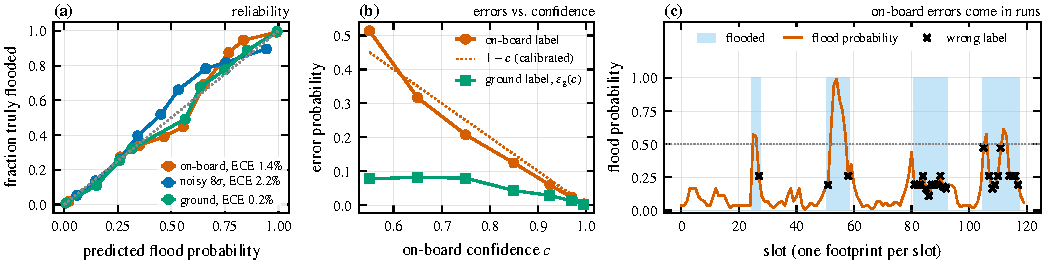
\includegraphics[width=\textwidth]{figures/fig_inference.pdf}
\caption{Inference traces on the Sen1Floods11 test chips. (a) Reliability diagram: fraction of flooded footprints versus the calibrated probability of flooding, for the on-board model, its noisiest variant (input noise of $8$ standard deviations), and the ground model, with expected calibration errors (ECE) in parentheses. (b) Error probability of the on-board label and of the ground label versus the on-board confidence $c$; the dotted line is $1-c$, which a calibrated model follows. (c) A segment of $120$ consecutive footprints of one test chip: flooded footprints are shaded, the line is the on-board flood probability, and the on-board errors (crosses) come in runs, mostly when a flooded area is missed.}
\label{fig:inference}
\end{figure*}

We collect these modeling choices in an assumption. It is used only to design the controller; the simulations in Section~\ref{sec:results} replay real classifier outputs, which do not satisfy it exactly.

\begin{assumption}[Inference model]\label{as:inf}
(i) The on-board classifier is calibrated, i.e.,~\eqref{eq:calib} holds. (ii) Given the source path, the on-board outputs $(\lab(t),c(t))$ are independent across slots. (iii) Given $X(t)$ and $c(t)=c$, the ground label is wrong with probability $\ee_{\rm g}(c)<\tfrac12$, independently of $\lab(t)$ and of the past.
\end{assumption}

Part (ii) is the strongest of the three. Consecutive footprints overlap by half, so a feature that fools the classifier in one frame tends to fool it in the next. Fig.~\ref{fig:inference}(c) shows such runs of errors. Over the validation and test chips, the on-board label is wrong in $8.2\%$ of the slots, but in $56\%$ of the slots that follow a wrong label, and a run of errors lasts $2.2$ slots on average. We keep part (ii) because it yields a tractable belief update, and we correct for its optimism in Section~\ref{sec:belief}. Assumption~\ref{as:inf} generalizes the semantic-noise model of Tiny-SEM~\cite{hosny2026tinysem}, in which the noise level is the same for every sample.

\subsection{Actions and Channel}\label{sec:act}
At the start of slot $t$, after classifying the frame, the UAV chooses an action $a(t)\in\A=\{0,1,2\}$. It stays silent ($a=0$), which costs nothing and leaves the GS status unchanged. It sends its label in a packet of $L_1$ bits ($a=1$), which corrects a wrong GS status if the label is right but makes a correct status wrong if the label is wrong. Or it uploads the frame in a packet of $L_2\gg L_1$ bits ($a=2$), so that the ground classifier labels it. In our scenario a label packet has $32$ bytes and a frame $50$ kilobytes. Whether a packet arrives, and how much energy it costs, depends on the link, which we model next.

Whether a packet arrives depends on the link state $g(t)=(\mathbf{u}(t),\beta(t))$. The first part is the position $\mathbf{u}(t)$ of the UAV on its route, which is known in advance because the route and the speed are fixed. The second part is a blockage indicator $\beta(t)\in\{0,1\}$. Buildings and terrain block the link for several slots at a time, so we model $\beta(t)$ as a two-state Markov chain with
\begin{equation}\label{eq:block}
\begin{split}
\Prob\big\{\beta(t+1)=1\mid\beta(t)=0\big\}&=\rho_{\rm b},\\
\Prob\big\{\beta(t+1)=0\mid\beta(t)=1\big\}&=\rho_{\rm u}.
\end{split}
\end{equation}
A blockage then lasts $1/\rho_{\rm u}$ slots on average, and a fraction $\rho_{\rm b}/(\rho_{\rm b}+\rho_{\rm u})$ of the slots is blocked. No packet gets through a blocked link.

When the link is not blocked, the received power depends on the distance $r$ between the UAV and the GS and on the elevation angle $\phi$. A low UAV is often seen through buildings, so the link is in line of sight (LoS) only with some probability. Following~\cite{alhourani2014lap}, we use the mean path loss
\begin{equation}\label{eq:pl}
\overline{\rm PL}(r,\phi)={\rm FSPL}(r)+P_{\rm LoS}(\phi)\,\eta_{\rm LoS}+\big(1-P_{\rm LoS}(\phi)\big)\eta_{\rm NLoS},
\end{equation}
where ${\rm FSPL}(r)$ is the free-space path loss, $\eta_{\rm LoS}$ and $\eta_{\rm NLoS}$ are the excess losses in LoS and non-LoS, and $P_{\rm LoS}(\phi)=[1+\alpha e^{-b(\phi-\alpha)}]^{-1}$ grows with the elevation angle, with environment constants $\alpha$ and $b$. The transmit power, the path loss~\eqref{eq:pl}, the bandwidth $W$ and the receiver noise figure give the mean signal-to-noise ratio (SNR) $\bar\gamma(g)$.

Small-scale fading makes the instantaneous SNR random around this mean. With Rayleigh fading, the instantaneous SNR is $\bar\gamma(g)\,|h|^2$ with $|h|^2$ exponentially distributed with unit mean. The fading coefficient $h$ stays constant during a slot. The UAV sends a packet of $L_a$ bits with a rateless (incremental-redundancy) code: it keeps sending coded bits until the GS decodes the packet and acknowledges it, or until a transmission window $\tau_{\max}\le\tau$ ends. Decoding takes the time $L_a/C(h)$, where $C(h)=W\log_2(1+\bar\gamma|h|^2)$ is the capacity of the faded channel, so the packet is decoded if $L_a/C(h)\le\tau_{\max}$, that is, if $W\tau_{\max}\log_2(1+\bar\gamma|h|^2)\ge L_a$. Solving for $|h|^2$ gives the delivery probability
\begin{equation}\label{eq:succ}
q_a(g)=(1-\beta)\,\exp\!\Big(-\frac{\gamma_a}{\bar\gamma(g)}\Big),\qquad \gamma_a=2^{L_a/(W\tau_{\max})}-1,
\end{equation}
for $a\in\{1,2\}$,
and $q_0\equiv0$. Here $\gamma_a$ is the SNR needed to deliver $L_a$ bits within the window. Since $L_2>L_1$, $\gamma_2>\gamma_1$, so $q_2(g)\le q_1(g)$ in every link state. In our scenario a label gets through almost surely whenever the link is not blocked, while a raw frame succeeds with probability between $0.99$ near the GS and $0.25$ at the far end of the trajectory.

The link is therefore an erasure channel: a packet either arrives intact or is lost, and a lost packet leaves the GS status unchanged. The link never changes the content of a label. Every packet carries a $32$-bit cyclic redundancy check (CRC), and the GS discards a packet whose check fails; a corrupted packet passes with probability about $2^{-32}$. We also assume that acknowledgments, which are short and sent by the GS at higher power, always arrive.

\begin{remark}[Undetected errors]\label{rem:flip}
Suppose instead that a decoded label is flipped with a small probability $\ee_{\rm u}$. Because the label is binary, a flipped disagreeing label equals the current GS status, so it changes nothing. A bit error on the link can therefore cancel an update but cannot make a correct GS status wrong. Its only effect is to replace $q_1(g)$ by $q_1(g)(1-\ee_{\rm u})$ in everything that follows. An undetected error in a raw frame corrupts the photo rather than the label, and its effect can be folded into the ground error $\ee_{\rm g}(c)$.
\end{remark}

\subsection{Energy Consumption}
A transmission costs the energy of the radio while it transmits plus a fixed overhead per packet. With the rateless code above, the radio is on for $\min\{L_a/C(h),\tau_{\max}\}$, so the expected energy of action $a$ is $P_{\rm r}\,\E_h\big[\min\{L_a/C(h),\tau_{\max}\}\big]+E_{\rm o}$. The controller needs this value before it transmits, when $h$ is unknown, and we approximate it by evaluating the airtime at the mean rate $\bar R(g)=W\log_2(1+\bar\gamma(g))$:
\begin{equation}\label{eq:energy}
E_a(g)=P_{\rm r}\min\Big\{\frac{L_a}{\bar R(g)},\tau_{\max}\Big\}+E_{\rm o},\quad a\in\{1,2\},
\end{equation}
and $E_0=0$. Here $P_{\rm r}$ is the power drawn by the radio and $E_{\rm o}$ is the overhead of waking up the radio, accessing the channel and receiving the acknowledgment. In our scenario a label costs about $20$\,mJ, almost all of it overhead, while a raw frame costs between $58$\,mJ and $420$\,mJ depending on the distance. Averaging over the fading instead gives $20$ to $22$\,mJ for a label and $64$ to $395$\,mJ for a raw frame along our trajectory. The approximation~\eqref{eq:energy} is thus accurate for labels and within $-30\%$ to $+12\%$ of the exact value for raw frames; it underestimates the cost of a raw frame most at intermediate distances, where a deep fade can extend the transmission to the full window. Capture, inference and propulsion~\cite{zeng2019rotary} cost the same whatever the decision, so we constrain only the communication energy, through a long-run average budget of $\bar E$ joules per slot:
\begin{equation}\label{eq:budget}
\limsup_{T\to\infty}\frac1T\sum_{t=0}^{T-1}\E\Big[E_{a(t)}\big(g(t)\big)\Big]\le\bar E.
\end{equation}
The expectation is over the action and the link state, which are random: they depend on the scene, the classifier outputs, the blockage and the past deliveries. Since $E_a(g)$ already averages over the fading, \eqref{eq:budget} limits the long-run average energy that the radio draws, up to the approximation error of~\eqref{eq:energy}. The $\limsup$ is needed because the running average need not converge for every policy. An average budget allows the UAV to spend more in some parts of the mission, for example near the GS where uploads are cheap, and less in others.

\subsection{The GS Status and the AoII}
Let $o(t)\in\{0,1\}$ indicate that the packet sent in slot $t$ is decoded, so $\Prob\{o(t)=1\mid a(t)=a,g(t)=g\}=q_a(g)$. The GS status, which we denote by $\hat X(t)$, is the most recent label the GS has received, whether it came from the UAV or from the ground classifier:
\begin{equation}\label{eq:est}
\hat X(t+1)=\begin{cases}\lab(t), & a(t)=1,\ o(t)=1,\\ \lab^{\rm g}(t), & a(t)=2,\ o(t)=1,\\ \hat X(t), & \text{otherwise.}\end{cases}
\end{equation}
Holding the last label is the natural estimator when the state is persistent ($p_x<\frac12$). The GS acknowledges every decoded packet and includes the new status $\hat X(t+1)$ in the acknowledgment, which costs one byte. The UAV therefore always knows $\hat X(t)$. It never knows $X(t)$.

The GS status can be wrong for two reasons. The scene may change, for example when the UAV passes from flooded patches to dry ones, while the GS keeps the old status until the UAV updates it. Or the update itself may be wrong: the small on-board classifier mislabels some photos, especially ambiguous ones such as a dry field after rain, and a wrong label that reaches the GS turns a correct status into a wrong one. What matters to the response teams is how long the status has been wrong: a status that is wrong for one slot does little harm, while one that is wrong for a minute may send a team to the wrong place. We therefore measure how well the GS knows the scene by the AoII~\cite{maatouk2020aoii}. The AoII is zero while the GS status is correct and counts the slots for which it has been wrong otherwise. After the scene moves to $X(t+1)$, it evolves as
\begin{equation}\label{eq:aoii}
\Delta(t+1)=\big(\Delta(t)+1\big)\,\ind{X(t+1)\neq\hat X(t+1)},\quad \Delta(0)=0.
\end{equation}
The AoII captures two effects that the AoI misses. A delivered wrong label makes a correct GS wrong, so the AoII starts to grow right after a delivery. A GS that has been wrong for a long time is penalized more than one that has just become wrong, which favors correcting long errors first.

Table~\ref{tab:aoiiex} gives an example from the flood scenario over eight slots. In slot $2$ a wrong ``flooded'' label is delivered, so the GS becomes wrong in slot $3$ although the scene has not changed. In slot $4$ the patch floods, and the GS happens to become correct. In slot $4$ the UAV also delivers a wrong ``dry'' label, so the GS is wrong again in slots $5$ and $6$, until a correct label sent in slot $6$ fixes it.

\begin{table}[t]
\caption{AoII in a flood example ($1$: flooded, $0$: dry)}\label{tab:aoiiex}
\centering\footnotesize
\setlength{\tabcolsep}{5pt}
\begin{tabular}{@{}lcccccccc@{}}
\toprule
Slot $t$ & 1 & 2 & 3 & 4 & 5 & 6 & 7 & 8\\
\midrule
True state $X(t)$ & 0 & 0 & 0 & 1 & 1 & 1 & 1 & 1\\
Delivered label in slot $t$ & -- & 1 & -- & 0 & -- & 1 & -- & --\\
GS status $\hat X(t)$ & 0 & 0 & 1 & 1 & 0 & 0 & 1 & 1\\
AoII $\Delta(t)$ & 0 & 0 & 1 & 0 & 1 & 2 & 0 & 0\\
\bottomrule
\end{tabular}
\end{table}

The AoII is random, since the scene, the on-board errors and the deliveries are, and it depends on the true state, which the UAV never observes. Section~\ref{sec:problem} therefore takes its long-run average as the objective and replaces it with a belief that the UAV can compute.

\subsection{Order of Events}\label{sec:events}
Within slot $t$, events occur in the following order.
\begin{enumerate}
\item The UAV observes the link state $g(t)$, captures $Y(t)$ and computes $\lab(t)$ and $c(t)$.
\item It chooses $a(t)$ and transmits if $a(t)\neq0$.
\item The packet is decoded with probability $q_{a(t)}(g(t))$. If it is, the GS updates its status by~\eqref{eq:est} and sends the acknowledgment.
\item The scene moves to $X(t+1)$, and the AoII becomes $\Delta(t+1)$ by~\eqref{eq:aoii}.
\end{enumerate}

%% =====================================================================
\section{Problem Formulation}\label{sec:problem}
%% =====================================================================
\subsection{Information and Policies}
When the UAV chooses $a(t)$, it knows its labels, confidences and link states up to slot $t$, and the outcome of every earlier transmission as reported by the acknowledgments,
\begin{equation}\label{eq:info}
\I(t)=\big\{\lab(s),c(s),g(s)\big\}_{s\le t}\cup\big\{a(s),\hat X(s+1)\big\}_{s<t},
\end{equation}
together with the ground label of every decoded upload.
It does not know the state $X(t)$ and therefore cannot compute the AoII $\Delta(t)$. A policy $\psi$ is a rule that maps the information $\I(t)$ to a probability distribution on the action set $\A$, from which $a(t)$ is drawn. We allow randomized policies because problems with an average constraint may need them to use the budget exactly. A transmission is pointless when the link is blocked, so we consider only policies with $a(t)=0$ whenever $q_1(g(t))=0$, and we denote their set by $\Psi$.

\subsection{The Optimization Problem}
The response teams need a GS status that is correct as often as possible and, when it is wrong, is corrected quickly. The long-run average AoII measures both: it grows with the fraction of slots in which the status is wrong, and it grows faster when the wrong periods are long, since the AoII counts the slots of each wrong period. Under a policy $\psi$, the average AoII and the average energy are
\begin{align}
\bar\Delta^{\psi}&=\limsup_{T\to\infty}\frac1T\sum_{t=0}^{T-1}\E^{\psi}\big[\Delta(t)\big],\label{eq:avgaoii}\\
\bar E^{\psi}&=\limsup_{T\to\infty}\frac1T\sum_{t=0}^{T-1}\E^{\psi}\Big[E_{a(t)}\big(g(t)\big)\Big],\label{eq:avgE}
\end{align}
where $\E^{\psi}$ is the expectation when the actions follow $\psi$, so that $\bar E^{\psi}$ is the left side of the budget~\eqref{eq:budget} under $\psi$. The UAV must keep the average AoII as low as possible without exceeding the budget:
\begin{equation}\label{eq:P}
\textbf{(P)}\qquad \min_{\psi\in\Psi}\ \bar\Delta^{\psi}\qquad\text{subject to}\qquad \bar E^{\psi}\le\bar E.
\end{equation}

Three features make (P) hard. First, it is partially observed: the cost $\Delta(t)$ depends on $X(t)$, which the UAV never sees, so the policy must act on its own inference about the state. Second, the cost has memory: by~\eqref{eq:aoii}, a wrong GS status adds to the AoII in every slot until it is corrected, so an action affects the cost of all the following slots, not only of the next one. Third, the energy constraint couples all slots: energy spent now is not available later, so the value of an update depends on the updates that the budget will allow in the future. The rest of this section deals with the first feature by replacing the unknown AoII with a probability distribution over its values, which turns (P) into a problem on a state that the UAV knows. Our policy handles the other two features approximately: Section~\ref{sec:structure} values each action by its effect on the AoII of the next slot, and Section~\ref{sec:lyap} enforces the budget online with a virtual queue that prices energy according to what has already been spent.

\subsection{A Belief on the AoII}\label{sec:belief}
The information $\I(t)$ grows without bound. The following lemma shows that a much smaller object carries everything the UAV needs to predict the AoII.

\begin{lemma}[Sufficient statistic]\label{lem:suff}
Given $\hat X(t)$, the AoII determines the state: $X(t)=\hat X(t)$ if $\Delta(t)=0$ and $X(t)=1-\hat X(t)$ if $\Delta(t)>0$. Hence the pair $(\hat X(t),\pi_t)$, where
\begin{equation}\label{eq:belief}
\pi_t(\delta)=\Prob\big\{\Delta(t)=\delta\mid\I(t)\big\},\qquad\delta\in\{0,1,\dots\},
\end{equation}
summarizes $\I(t)$ for predicting the future AoII.
\end{lemma}
\begin{proof}
By~\eqref{eq:aoii}, $\Delta(t)>0$ if and only if $X(t)\neq\hat X(t)$, and $X(t)$ is binary. So $(\hat X(t),\Delta(t))$ determines $X(t)$, and the future of $X$, $\hat X$ and $\Delta$ depends on the past only through $X(t)$, $\hat X(t)$ and $\Delta(t)$.
\end{proof}

The belief $\pi_t$ thus answers both questions at once. Its mass at $\delta=0$ is the probability that the GS is correct, and its mass at $\delta>0$ says how long the GS has probably been wrong. For a given $\delta$, we write $x_\delta$ for the state implied by Lemma~\ref{lem:suff}, i.e., $x_0=\hat X(t)$ and $x_\delta=1-\hat X(t)$ for $\delta>0$.

To store the belief with finite memory, we truncate its support at $\Delta_{\max}$ and keep any mass that would exceed $\Delta_{\max}$ at $\Delta_{\max}$. With $\Delta_{\max}=300$ the belief is a vector of $301$ numbers, about $1.2$\,kB in single precision. The mass at $\Delta_{\max}$ is negligible in all our experiments.

\subsection{Belief Update}
The belief changes for three reasons in each slot: the UAV sees a new on-board label, it may receive a ground label, and the scene evolves. Let $\pi^-_t$ denote the belief at the start of slot $t$, before the new frame is classified. The update has three steps.

\emph{Step 1: correction with the on-board label.} By Bayes' rule, the frame changes the belief in proportion to its likelihood under each value of the AoII:
\begin{equation}\label{eq:bayes}
\pi_t(\delta)\propto\pi^-_t(\delta)\,\Prob\big\{\lab(t),c(t)\mid\Delta(t)=\delta,\I(t-1)\big\}.
\end{equation}
Under Assumption~\ref{as:inf}(ii), the label and the confidence depend on the past only through the current state, which is $x_\delta$ by Lemma~\ref{lem:suff}. By~\eqref{eq:lik}, the likelihood in~\eqref{eq:bayes} is therefore proportional to $c_{x_\delta}(t)/\varpi_{x_\delta}$. All hypotheses $\delta>0$ imply the same state $1-\hat X(t)$, so the likelihood takes only two values, one if the GS is right ($\delta=0$) and one if it is wrong ($\delta>0$). Only their ratio matters. Let $d(t)=\ind{\lab(t)\neq\hat X(t)}$ indicate that the label disagrees with the GS. Their ratio is
\begin{equation}\label{eq:Lambda}
\Lambda_t=\frac{c_{1-\hat X(t)}(t)}{c_{\hat X(t)}(t)}\cdot\frac{\varpi_{\hat X(t)}}{\varpi_{1-\hat X(t)}},
\end{equation}
which says how many times more likely the frame is if the GS is wrong than if it is right. By~\eqref{eq:cx}, the first factor is $c(t)/(1-c(t))$ if the label disagrees with the GS and $(1-c(t))/c(t)$ if it agrees. A label that disagrees with the GS thus has $\Lambda_t$ increasing in its confidence: it is evidence that the GS is wrong, and the more so the more confident it is. A label that agrees with the GS is evidence that the GS is right.

Exact Bayes' rule would multiply the mass at $\delta>0$ by $\Lambda_t$ relative to the mass at $\delta=0$. This treats every frame as an independent observation, which overstates the evidence when errors come in runs. If a frame overlaps half of the previous one and the classifier missed the flood in the previous frame, a second miss is far from independent confirmation (Fig.~\ref{fig:inference}(c)). We therefore temper the ratio with an exponent $\nu\in(0,1]$. With $\mu^-_t=\pi^-_t(\Delta>0)$ the prior probability that the GS is wrong, the corrected belief is
\begin{equation}\label{eq:post}
\pi_t(\delta)=\frac{\pi^-_t(\delta)}{1-\mu^-_t+\mu^-_t\Lambda_t^{\nu}}\times\begin{cases}1, & \delta=0,\\ \Lambda_t^{\nu}, & \delta>0.\end{cases}
\end{equation}
The exponent counts each frame as a fraction $\nu$ of an independent observation, and $\nu=1$ recovers Bayes' rule. A rough guide is the inverse of the mean length of an error run: our on-board errors last $2.2$ slots on average, which suggests $\nu\approx0.45$. In the evaluation we select $\nu\in\{0.25,0.5\}$ on tuning data together with the other parameters of the controller. We also include, as an option, the symmetric update that ignores the prior and uses $\varpi_0=\varpi_1$ with $\nu=1$, in which the confidence itself is the likelihood.

Step 1 multiplies the odds that the GS is wrong by $\Lambda_t^{\nu}$. It moves mass between ``the GS is right'' and ``the GS is wrong'' but does not change the shape of the belief within $\delta>0$.

\emph{Step 2: correction with the ground label.} If the UAV uploaded the frame and the GS decoded it, the acknowledgment carries the ground label, and~\eqref{eq:post} is applied once more with $\nu=1$. Its error probability $\ee_{\rm g}=\ee_{\rm g}(c(t))$ is defined given the state, so no prior correction is needed, and the ratio is $(1-\ee_{\rm g})/\ee_{\rm g}$ if the ground label disagrees with $\hat X(t)$ and $\ee_{\rm g}/(1-\ee_{\rm g})$ otherwise.

\emph{Step 3: prediction.} After the transmission, the GS holds $\xh'=\hat X(t+1)$, which the UAV knows from the acknowledgment or from the absence of one. For each $\delta$, the state $X(t)=x_\delta$ is known, so the UAV knows whether the GS status is now correct for that hypothesis. By~\eqref{eq:aoii}, the AoII grows to $\delta+1$ if $X(t+1)\neq\xh'$ and resets to 0 otherwise. If $x_\delta=\xh'$, the status becomes wrong only if the state changes, which happens with probability $p_{x_\delta}$. If $x_\delta\neq\xh'$, it stays wrong if the state does not change, with probability $1-p_{x_\delta}$. Hence
\begin{equation}\label{eq:pred}
\Prob\big\{\Delta(t+1)=\delta+1\mid\Delta(t)=\delta\big\}=\begin{cases}p_{x_\delta}, & x_\delta=\xh',\\ 1-p_{x_\delta}, & x_\delta\neq\xh',\end{cases}
\end{equation}
with $\Delta(t+1)=0$ otherwise. Summing over $\delta$ under $\pi_t$ gives $\pi^-_{t+1}$. A delivered label that flips the GS status swaps the two cases of~\eqref{eq:pred}, which is how a correction moves the mass of the belief back towards $\delta=0$.

Two summaries of the belief appear in the rest of the paper:
\begin{equation}\label{eq:musum}
\mu_t=\pi_t(\Delta>0),\qquad S_t=\E_{\pi_t}\big[(\Delta+1)\ind{\Delta>0}\big].
\end{equation}
The first is the probability that the GS is wrong. The second weighs each wrong hypothesis by the AoII it will have in the next slot if the GS stays wrong. We write $\mu^-_t$ and $S^-_t$ for the same summaries of $\pi^-_t$.

\subsection{A Worked Example}
\begin{example}\label{ex:belief}
Let the GS report ``not flooded'' ($\hat X(t)=0$), and let the UAV hold the belief $\pi^-_t(0)=0.95$, $\pi^-_t(1)=0.05$: it is fairly sure the GS is right. A frame then arrives with label ``flooded'' and confidence $c=0.9$, so $d(t)=1$. With $\varpi_0=0.81$ and $\varpi_1=0.19$,~\eqref{eq:Lambda} gives $\Lambda_t=(0.81/0.19)(0.9/0.1)=38.4$: the frame is $38$ times more likely if the GS is wrong. With exact Bayes' rule ($\nu=1$),~\eqref{eq:post} gives $\mu_t=0.05\cdot38.4/(0.95+0.05\cdot38.4)=0.67$: one confident frame makes the GS more likely wrong than right. With $\nu=0.5$ the same frame gives only $\mu_t=0.25$, and with $\nu=0.25$ it gives $\mu_t=0.12$. Suppose the UAV stays silent. The prediction~\eqref{eq:pred} with $p_0=0.039$ and $p_1=0.166$ gives $\mu^-_{t+1}=0.23$ for $\nu=0.5$. If the next frame again says ``flooded'' with $c=0.9$, the belief rises to $\mu_{t+1}=0.65$. With the tempered update, the UAV therefore needs two consistent frames to become as convinced as one frame makes it under exact Bayes' rule. Section~\ref{sec:structure} continues this example to show what the UAV does in each of these two slots.
\end{example}

\subsection{Equivalent Belief-State Problem and Solution Approach}
By Lemma~\ref{lem:suff}, (P) is equivalent to a constrained Markov decision process whose state is the belief together with the observable quantities, $(\pi^-_t,\hat X(t),\lab(t),c(t),g(t))$. The per-slot cost is the expected AoII $\E[\Delta(t+1)\mid\I(t),a(t)]$, which the belief gives, and the per-slot energy is $E_{a(t)}(g(t))$. The transition kernel follows from the model: the next label and confidence are drawn from their law given $X(t+1)$; $g(t+1)$ follows the trajectory and the blockage chain~\eqref{eq:block}; $\hat X(t+1)$ follows~\eqref{eq:est}; and $\pi^-_{t+1}$ follows the three steps of Section~\ref{sec:belief}.

The standard approach prices the energy constraint with a Lagrange multiplier $\lambda\ge0$, solves the unconstrained problem with per-slot cost $\E[\Delta(t+1)]+\lambda E_{a(t)}(g(t))$ by value iteration, and searches over $\lambda$ to meet the budget. This is impractical on a UAV: the belief is a point in a high-dimensional simplex, the kernel needs the law of the confidence, the blockage statistics and the trajectory, which change between missions, and the right multiplier depends on all of them. We therefore take a different route. Section~\ref{sec:structure} characterizes the value of each action in one slot in closed form, and Section~\ref{sec:lyap} builds an online policy on this characterization, with an energy price that adapts to the energy actually spent.

%% =====================================================================
\section{The Value of Each Action}\label{sec:structure}
%% =====================================================================
Any reasonable policy must compare, in each slot, how much each action is expected to lower the AoII with how much energy it costs. This section derives the first quantity in closed form and shows what it implies for the decision. Throughout, we fix slot $t$, let $\xh=\hat X(t)$, and write
\begin{equation}\label{eq:rw}
r=p_{\xh},\qquad w=p_{1-\xh}.
\end{equation}
In words, $r$ is the probability that the state leaves the value the GS currently reports, and $w$ is the probability that it leaves the other value. By~\eqref{eq:source}, both are below $\frac12$.

\subsection{One-Step Expected AoII}
We first compute the expected AoII in slot $t+1$ for a given hypothesis $\Delta(t)=\delta$ and a given new status $\xh'=\hat X(t+1)$. By~\eqref{eq:aoii}, $\Delta(t+1)$ is either $\delta+1$ or $0$, so its expectation is $\delta+1$ times the probability in~\eqref{eq:pred}: $(\delta+1)p_{x_\delta}$ if the new status equals $x_\delta$, and $(\delta+1)(1-p_{x_\delta})$ otherwise. The three actions differ only in which status $\xh'$ they produce, and with what probability. We evaluate this expectation for each of them, assuming the packet is delivered, and average it over $\pi_t$.

\emph{Silence.} The status stays $\xh'=\xh$. If $\delta=0$, then $x_0=\xh=\xh'$ and the probability is $p_{\xh}=r$. If $\delta>0$, then $x_\delta=1-\xh\neq\xh'$ and the probability is $1-p_{1-\xh}=1-w$. Averaging over $\pi_t$ and using~\eqref{eq:musum},
\begin{equation}\label{eq:J0}
J_0=(1-\mu_t)\,r+S_t\,(1-w).
\end{equation}

\emph{Label.} If $d(t)=0$, the label equals $\xh$ and changes nothing, so the result is $J_0$. If $d(t)=1$, a delivered label flips the GS status to $\xh'=1-\xh$. Now the case $\delta=0$ has $x_0\neq\xh'$ and probability $1-r$, and the case $\delta>0$ has $x_\delta=\xh'$ and probability $w$, so
\begin{equation}\label{eq:J1}
J_1=(1-\mu_t)(1-r)+S_t\,w.
\end{equation}

\emph{Raw upload.} The ground label equals $X(t)$ with probability $1-\ee_{\rm g}$, where $\ee_{\rm g}=\ee_{\rm g}(c(t))$, and by Assumption~\ref{as:inf}(iii) this event is independent of $\Delta(t)$ given $c(t)$. If the ground label is correct, then $\xh'=x_\delta$ and the probability is $p_{x_\delta}$, which is $r$ for $\delta=0$ and $w$ for $\delta>0$. If it is wrong, the probability is $1-p_{x_\delta}$. Mixing the two cases,
\begin{equation}\label{eq:J2}
J_2=(1-\mu_t)\big[r+\ee_{\rm g}(1-2r)\big]+S_t\big[w+\ee_{\rm g}(1-2w)\big].
\end{equation}

A transmission is delivered with probability $q_a(g)$ and has no effect otherwise, and delivery is independent of the scene given $g$. The expected AoII after action $a$ is therefore $(1-q_a)J_0+q_aJ_a=J_0-q_a(J_0-J_a)$. We call the difference $G_a=J_0-J_a$ the gain of action $a$: it is the reduction in the expected AoII of the next slot that a delivered packet of type $a$ brings. Subtracting~\eqref{eq:J1} and~\eqref{eq:J2} from~\eqref{eq:J0} proves the following lemma.

\begin{lemma}[One-step expected AoII]\label{lem:onestep}
Under Assumption~\ref{as:inf}, $\E[\Delta(t+1)\mid\I(t),a(t)=a]=J_0-q_a(g)\,G_a$, with $G_0=0$ and
\begin{align}
G_1&=\big[S_t(1-2w)-(1-\mu_t)(1-2r)\big]\,d(t), \label{eq:G1}\\
G_2&=(1-\ee_{\rm g})\,S_t(1-2w)-\ee_{\rm g}\,(1-\mu_t)(1-2r). \label{eq:G2}
\end{align}
\end{lemma}

Both gains are built from the same two terms. The term $S_t(1-2w)$ is the AoII that an update removes when the GS is wrong and the update is right. The term $(1-\mu_t)(1-2r)$ is the AoII that an update creates when the GS is right and the update is wrong. Since $r,w<\frac12$, both terms are nonnegative. A delivered disagreeing label removes the first term in full, because a label that disagrees with a wrong GS is necessarily correct. It also creates the second in full, because a label that disagrees with a correct GS is necessarily wrong. A ground label removes the first term only with probability $1-\ee_{\rm g}$, but it creates the second only with probability $\ee_{\rm g}$. The label is therefore a bold update and the raw upload a cautious one. A label that is probably wrong has $G_1<0$ and would increase the expected AoII, while the raw upload has $G_2>0$ as soon as $S_t(1-2w)(1-\ee_{\rm g})>\ee_{\rm g}(1-\mu_t)(1-2r)$, which holds even for a small probability that the GS is wrong when the ground classifier is accurate.

\setcounter{example}{0}
\begin{example}[continued]
In slot $t$ of Example~\ref{ex:belief} with $\nu=0.5$, the belief is $\mu_t=0.25$ and $S_t=0.49$, and the ground error at $c=0.9$ is $\ee_{\rm g}=0.028$ (Fig.~\ref{fig:inference}(b)). With $\xh=0$, $r=p_0=0.039$ and $w=p_1=0.166$. Lemma~\ref{lem:onestep} gives $G_1=-0.37$ and $G_2=0.30$: sending the label would more likely harm than help, while asking the ground would help. In slot $t+1$, after the second disagreeing frame, $\mu_{t+1}=0.65$ and the gains become $G_1=0.94$ and $G_2=1.21$. Now the GS is probably wrong, and the label is worth sending.
\end{example}

For a symmetric source the gains take a simpler form, in terms of the mean of the belief.

\begin{corollary}[Symmetric source]\label{cor:sym}
If $p_0=p_1=p$, then with $\Dbar_t=\E_{\pi_t}[\Delta(t)]$,
\begin{align*}
G_1&=(1-2p)\big(\Dbar_t+2\mu_t-1\big)\,d(t),\\
G_2&=(1-2p)\big(\mu_t+(1-\ee_{\rm g})\Dbar_t-\ee_{\rm g}\big).
\end{align*}
\end{corollary}
\begin{proof}
With $r=w=p$, both terms of the gains carry the factor $1-2p$. Since $S_t=\E_{\pi_t}[\Delta\ind{\Delta>0}]+\mu_t=\Dbar_t+\mu_t$, substituting in~\eqref{eq:G1} and~\eqref{eq:G2} gives the result.
\end{proof}

Corollary~\ref{cor:sym} gives a simple test for the label: a disagreeing label lowers the expected AoII if and only if $\Dbar_t+2\mu_t>1$. When the GS has just become wrong, $\Dbar_t\approx\mu_t$, and the test reduces to $\mu_t>\frac13$. As the GS stays wrong, $\Dbar_t$ grows and a smaller probability of error suffices. The test does not depend on $p$, since the factor $1-2p$ only scales both gains.

\subsection{Agreeing Labels}
The gains also show which updates are never useful.

\begin{proposition}[No confirmations]\label{prop:confirm}
If $d(t)=0$, then $G_1=0$. Hence a policy that minimizes the expected AoII plus a nonnegative energy price never needs to send a label that agrees with the GS.
\end{proposition}
\begin{proof}
If $d(t)=0$, a delivered label leaves the status unchanged, so $J_1=J_0$ and $G_1=0$. Sending it then costs $E_1(g)>0$ and changes nothing else, so silence does at least as well for any energy price $\lambda\ge0$.
\end{proof}

Proposition~\ref{prop:confirm} rules out a common design, in which the device reports every label so that the receiver can confirm its status: the GS acts only on its status, which a confirmation does not change, and the UAV already knows the label. The pre-identification baseline of Section~\ref{sec:results} spends most of its energy on such labels.

\subsection{Threshold Structure of the Per-Slot Decision}
Lemma~\ref{lem:onestep} measures the value of an action in AoII, while its cost is measured in energy. A per-slot rule must convert one into the other. We consider rules of the form
\begin{equation}\label{eq:rule}
a(t)\in\arg\max_{a\in\A}\big\{V\,q_a(g)\,G_a-\lambda(t)\,E_a(g)\big\},
\end{equation}
where $V>0$ weighs the AoII and $\lambda(t)\ge0$ is a price per joule that may change over time. Section~\ref{sec:lyap} shows that the drift-plus-penalty method produces exactly this rule, with $\lambda(t)$ equal to an energy debt. Here we ask how the decision depends on the confidence of the frame.

The confidence enters the gains only through the belief $\pi_t$, and by~\eqref{eq:post} only through the ratio $\Lambda_t$. By~\eqref{eq:Lambda}, $\Lambda_t$ increases in $c$ if $d(t)=1$ and decreases in $c$ if $d(t)=0$. The next lemma shows that both gains, and any nonnegative combination of their two terms, increase with $\Lambda_t$.

\begin{lemma}[Monotonicity in the evidence]\label{lem:mono}
Fix $\pi^-_t$. For any $A,B\ge0$, the quantity $AS_t-B(1-\mu_t)$ is a nondecreasing function of $\Lambda_t$.
\end{lemma}

The proof is in Appendix~\ref{app:mono}. Combined with Lemma~\ref{lem:onestep}, it yields the structure of the decision.

\begin{proposition}[Confidence thresholds]\label{prop:threshold}
Let $\ee_{\rm g}$ be constant, and fix $\pi^-_t$, $\hat X(t)$, $g$ and $\lambda(t)$.
\begin{enumerate}
\item[(a)] If $d(t)=1$, there are thresholds $c_{\rm r}\le c_{\lab}$ such that~\eqref{eq:rule} stays silent for $c<c_{\rm r}$, uploads the frame for $c_{\rm r}\le c<c_{\lab}$, and sends the label for $c\ge c_{\lab}$. Any of the three intervals may be empty.
\item[(b)] If $d(t)=0$, it uploads the frame if and only if $c\le c^0_{\rm r}$ for some threshold $c^0_{\rm r}$, and stays silent otherwise.
\item[(c)] For fixed $\mu^-_t$, the silent regions shrink as $S^-_t$ grows, and they grow with $\lambda(t)$.
\end{enumerate}
\end{proposition}

The proof is in Appendix~\ref{app:threshold}. Part (a) is the rule of the title. A frame that disagrees with the GS is sent as a label when the UAV is sure of it, sent to the ground when the UAV is unsure, and withheld when it is too unsure for either to pay off. Part (b) says that a frame that agrees with the GS can still be worth uploading, but only if it is unsure: an unsure agreement leaves room for the GS to be wrong, and the ground classifier can check. Part (c) says that the UAV becomes more willing to act the longer the GS has probably been wrong, and less willing as energy becomes more expensive.

\setcounter{example}{0}
\begin{example}[continued]
Let the UAV be $1.2$\,km from the GS, where $q_1\approx1$, $q_2=0.78$, $E_1=20$\,mJ and $E_2=190$\,mJ. In slot $t$, the label has $q_1G_1<0$, and the upload has $q_2G_2=0.23$, so~\eqref{eq:rule} uploads the frame if $\lambda/V<0.23/0.19=1.2$\,J$^{-1}$ and stays silent otherwise. In slot $t+1$, $q_1G_1=0.94$ and $q_2G_2=0.95$ are almost equal, but the label costs a tenth of the upload, so the UAV sends the label for any price between about $0.05$ and $47$\,J$^{-1}$. At the price $\lambda/V=2$\,J$^{-1}$ used in Fig.~\ref{fig:regions}, the UAV thus waits in slot $t$ and sends the label in slot $t+1$.
\end{example}

\begin{figure}[t]
\centering
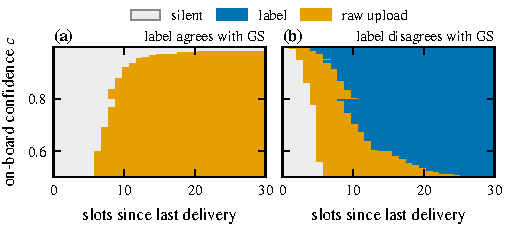
\includegraphics[width=\columnwidth]{figures/regions.pdf}
\caption{Decisions of~\eqref{eq:rule} versus the slots since the last delivery and the confidence, with parameters estimated on Sen1Floods11: GS reports ``not flooded'' with $5\%$ initial doubt, UAV $1.2$\,km from the GS ($q_1\approx1$, $q_2=0.78$, $E_1=20$\,mJ, $E_2=190$\,mJ), $\lambda/V=2$\,J$^{-1}$, $\nu=0.25$. The steps at $c=0.8$ and $c=0.9$ come from the binned estimate of $\ee_{\rm g}(c)$.}
\label{fig:regions}
\end{figure}

Fig.~\ref{fig:regions} shows the decision regions of~\eqref{eq:rule} for the scenario of the example, as a function of the slots since the last delivery and of the confidence. It uses the confidence-dependent $\ee_{\rm g}(c)$ estimated from our data, which Proposition~\ref{prop:threshold} does not cover; the order silent, raw, label still holds. When the label disagrees with the GS, the confidence needed to send it falls as the GS status ages, because the prior probability that the GS is wrong grows. When the label agrees with the GS but is unsure, the UAV uploads the frame once the status is old enough, which amounts to asking the GS to verify its status.

%% =====================================================================
\section{Online Policy: CA-DPP}\label{sec:lyap}
%% =====================================================================
The rule~\eqref{eq:rule} needs an energy price $\lambda(t)$. A fixed price would have to be tuned to the mission, and a wrong value either wastes the budget or leaves it unused. This section derives a price from the energy actually spent, using Lyapunov drift-plus-penalty~\cite{neely2010book}, and shows that the resulting policy meets the budget.

\subsection{Energy Debt as a Virtual Queue}
We track how far the UAV has spent beyond its budget with a virtual queue,
\begin{equation}\label{eq:Z}
Z(t+1)=\max\Big\{Z(t)+E_{a(t)}\big(g(t)\big)-\bar E,\ 0\Big\},\qquad Z(0)=0.
\end{equation}
In each slot the queue grows by the energy spent and drains by the budget, so $Z(t)$ is the energy debt of the UAV. Since $\max\{z,0\}\ge z$, summing~\eqref{eq:Z} over $t<T$ gives $Z(T)\ge\sum_{t<T}\big(E_{a(t)}(g(t))-\bar E\big)$, or
\begin{equation}\label{eq:Zbound}
\frac1T\sum_{t=0}^{T-1}E_{a(t)}\big(g(t)\big)\le\bar E+\frac{Z(T)}{T}.
\end{equation}
Hence the budget~\eqref{eq:budget} holds whenever the debt grows slower than linearly. The policy should therefore keep $Z(t)$ small while it keeps the AoII low.

\subsection{Drift-Plus-Penalty}
To keep the queue small, we measure its size by $L(t)=\frac12Z(t)^2$ and its expected growth in one slot by the drift $\E[L(t+1)-L(t)\mid\I(t)]$. Squaring~\eqref{eq:Z} and using $\max\{z,0\}^2\le z^2$,
\[
Z(t+1)^2\le Z(t)^2+\big(E_{a(t)}-\bar E\big)^2+2Z(t)\big(E_{a(t)}-\bar E\big).
\]
The middle term is at most $\max\{E_{\max},\bar E\}^2$, where $E_{\max}=\max_{a,g}E_a(g)$. Taking conditional expectations,
\begin{equation}\label{eq:drift}
\E\big[L(t+1)-L(t)\,|\,\I(t)\big]\le C+Z(t)\,\E\Big[E_{a(t)}\big(g(t)\big)-\bar E\,\big|\,\I(t)\Big],
\end{equation}
with $C=\frac12\max\{E_{\max},\bar E\}^2$. The drift-plus-penalty method chooses, in each slot, the action that minimizes the right-hand side of~\eqref{eq:drift} plus $V$ times the expected penalty, here the expected AoII of the next slot. By Lemma~\ref{lem:onestep}, this is
\[
\min_{a\in\A}\Big\{Z(t)E_a(g)+V\big(J_0-q_a(g)G_a\big)\Big\}.
\]
The terms $C$, $Z(t)\bar E$ and $VJ_0$ do not depend on the action, so the minimization is equivalent to~\eqref{eq:rule} with $\lambda(t)=Z(t)$. The energy price is thus the energy debt. When the UAV has spent more than its budget, energy becomes expensive and the silent regions of Proposition~\ref{prop:threshold}(c) grow. When it has spent less, the debt drains to zero and every useful update is sent.

We call the resulting policy confidence-aware drift-plus-penalty (CA-DPP). Algorithm~\ref{alg:dpp} lists its steps.

\begin{algorithm}[t]
\caption{CA-DPP, executed by the UAV in slot $t$}\label{alg:dpp}
\begin{algorithmic}[1]
\State Classify $Y(t)$ to get $\lab(t)$, $c(t)$; observe $g(t)$; set $d(t)$
\State Correct $\pi^-_t\to\pi_t$ by~\eqref{eq:post}; compute $\mu_t$, $S_t$
\State Compute $G_1$, $G_2$ by~\eqref{eq:G1}--\eqref{eq:G2}
\If{$q_1(g(t))=0$} $a(t)\gets0$
\Else\ $a(t)\gets\arg\max_a\{Vq_a(g)G_a-Z(t)E_a(g)\}$, ties to silence
\EndIf
\State Transmit; read the acknowledgment: $\hat X(t+1)$, and $\lab^{\rm g}(t)$ after a decoded raw upload
\State If a ground label arrived, correct $\pi_t$ with it (Step 2)
\State Predict $\pi^-_{t+1}$ by~\eqref{eq:pred}
\State $Z(t+1)\gets\max\big\{Z(t)+E_{a(t)}(g(t))-\bar E,0\big\}$
\end{algorithmic}
\end{algorithm}

\subsection{Energy Guarantee}
The next theorem shows that CA-DPP keeps the energy debt bounded on every sample path, so it meets the budget without any knowledge of the statistics of the scene, the classifier or the link.

\begin{theorem}[Budget]\label{thm:budget}
Let $E_{\min}=\min_{a\neq0,g}E_a(g)>0$. Under CA-DPP, for every sample path and every $t$,
\begin{equation}\label{eq:Zmax}
Z(t)\le Z_{\max}=\frac{V(\Delta_{\max}+1)}{E_{\min}}+E_{\max}.
\end{equation}
Consequently, $\frac1T\sum_{t<T}E_{a(t)}(g(t))\le\bar E+Z_{\max}/T$ for every $T$, and~\eqref{eq:budget} holds.
\end{theorem}

The proof is in Appendix~\ref{app:budget}. A gain never exceeds $\Delta_{\max}+1$, so once $Z(t)E_a(g)$ exceeds $V(\Delta_{\max}+1)$ for every transmission, the UAV stays silent and the debt drains. The bound~\eqref{eq:Zmax} is loose; it shows that the budget is met by construction, while in our experiments the energy spent stays within $5\%$ of the budget.

\subsection{Complexity and Parameters}
A slot of CA-DPP costs $O(\Delta_{\max})$ operations, a few hundred multiply-adds for $\Delta_{\max}=300$, which is less than one inference of the on-board classifier. The memory is the belief vector, about $1.2$\,kB, plus small tables of $\ee_{\rm g}(c)$, $q_a(g)$ and $E_a(g)$.

CA-DPP has two parameters. The weight $V$ trades the AoII against the size of the energy debt: a larger $V$ lowers the AoII but lets the debt grow larger before it brakes the UAV, so the energy spent over a finite mission exceeds the budget by more (Section~\ref{sec:results}). The exponent $\nu$ sets how much each frame moves the belief. Both are chosen on tuning data before the mission. The statistics that CA-DPP uses, namely $p_0$, $p_1$, $\varpi$ and $\ee_{\rm g}(c)$, are estimated on the same data.

\subsection{Extensions and Performance}
\begin{remark}[Harvesting battery]\label{rem:harvest}
Suppose the UAV, or a ground sensor that runs the same policy, harvests energy into a battery of finite capacity, and let $B(t)$ be the energy stored in slot $t$. The constraint is then that the battery never runs empty, instead of~\eqref{eq:budget}. The perturbed Lyapunov method of~\cite{huang2013eh} applies the same derivation to the battery, shifted by a constant $\theta$, and yields~\eqref{eq:rule} with $\lambda(t)=\theta-B(t)$: energy becomes expensive when the battery is low. By the argument behind Theorem~\ref{thm:budget}, choosing $\theta\ge E_{\max}+V(\Delta_{\max}+1)/E_{\min}$ ensures that the UAV never chooses an action that the battery cannot pay for.
\end{remark}

\begin{remark}[Optimality]\label{rem:opt}
For problems in which the per-slot cost depends only on the current state and action, drift-plus-penalty comes within $O(1/V)$ of the optimal cost~\cite{neely2010book}. This bound does not apply here, because the AoII depends on past decisions through the GS status, and CA-DPP minimizes only the AoII of the next slot. A version that applies~\eqref{eq:rule} between deliveries, instead of in every slot, fits the renewal framework of~\cite{neely2013renewal}, in which each delivery starts a new frame. Deriving a performance bound for that version is left to future work. Section~\ref{sec:results} compares CA-DPP with a genie that knows the state, which indicates how much room for improvement remains.
\end{remark}

%% =====================================================================
\section{Trace-Driven Evaluation}\label{sec:results}
%% =====================================================================
We evaluate CA-DPP on real classifier outputs, replayed over a simulated air-to-ground link. Replaying real outputs matters here: the on-board errors in the traces are correlated in time and only approximately calibrated, so they test the policy under conditions that violate Assumption~\ref{as:inf}.

\subsection{Data}
We build the traces from the hand-labeled part of Sen1Floods11~\cite{bonafilia2020sen1floods11}. It contains 446 Sentinel-2 chips of $512\times512$ pixels at $10$\,m resolution from eleven flood events on several continents, with per-pixel water labels and official train, validation and test splits. No UAV flood dataset with pixel labels of comparable size exists, so this imagery stands in for the UAV view.

To turn a chip into a sequence of frames, a $64\times64$-pixel footprint scans the chip along a serpentine path with a stride of $32$ pixels, one footprint per slot. Consecutive footprints therefore overlap by half, as consecutive frames of a UAV flying at constant speed would. This scan gives the sequence of photos; the position of the UAV, which sets the link, follows the route described below and is generated separately (see Section~\ref{sec:discussion}). A footprint is labeled flooded if at least $10\%$ of its labeled pixels are water, and footprints with less than $80\%$ labeled pixels are skipped. This leaves $46{,}774$, $16{,}612$ and $16{,}811$ slots in the train, validation and test splits. The resulting state sequence is strongly correlated: on the training split, $p_0=0.039$ and $p_1=0.166$, so a dry stretch lasts $26$ slots on average and a flooded stretch $6$ slots.

\subsection{Classifiers}
The on-board model must fit a small processor. We use a logistic regression on the $8\times8$ average-pooled blue, green, red and near-infrared bands, which has $257$ parameters. The ground model can be much larger. We use a gradient-boosted tree ensemble with $300$ trees on $77$ statistics of all $13$ bands and two water indices. Both models are trained on the training split and calibrated by isotonic regression on the validation split.

To study weaker on-board models, we add Gaussian noise of $2$, $4$, $6$ and $8$ times the per-band standard deviation to the input of the on-board model and recalibrate it. On the $174$ validation and test chips ($33{,}423$ slots, $20.5\%$ of them flooded), the five on-board variants are correct on $91.8\%$, $89.4\%$, $86.7\%$, $83.9\%$ and $81.8\%$ of the slots, and the ground model on $97.6\%$. The noise also makes the on-board errors lopsided: the noisiest variant labels $7\%$ of the test slots as flooded, against $21\%$ in truth, so most of its errors are missed floods. Calibration keeps its confidences honest (Fig.~\ref{fig:inference}(a)), so a calibrated controller can still tell when such a model is unsure.

\subsection{Scenario}
Table~\ref{tab:params} lists the scenario parameters. Over one orbit of $200$\,s, the distance to the GS ranges from $0.2$ to $2.8$\,km. The link parameters give a label energy of about $20$\,mJ everywhere and a raw upload that costs $58$ to $420$\,mJ and succeeds with probability $0.99$ to $0.25$, depending on the distance. Blockage has $\rho_{\rm b}=0.02$ and $\rho_{\rm u}=0.1$, so $17\%$ of the slots are blocked, for $10$ slots on average. We consider budgets $\bar E$ from $0.25$ to $10$\,mJ per slot. At the lowest budget the UAV can afford a label in about one slot in $80$, and at the highest it can afford a raw upload in most slots near the GS.

\begin{table}[t]
\caption{Scenario parameters}\label{tab:params}
\centering\footnotesize
\begin{tabular}{@{}ll@{}}
\toprule
Parameter & Value\\
\midrule
Slot length $\tau$; transmission window $\tau_{\max}$ & $0.5$\,s; $0.4$\,s\\
UAV altitude; orbit radius; center to GS & $100$\,m; $1.3$\,km; $1.5$\,km\\
Orbit period & $400$ slots\\
Carrier; bandwidth $W$; transmit power & $2.4$\,GHz; $1$\,MHz; $20$\,dBm\\
Noise figure; environment & $7$\,dB; urban~\cite{alhourani2014lap}\\
Blockage $\rho_{\rm b}$; $\rho_{\rm u}$ & $0.02$; $0.1$\\
Label size $L_1$; frame size $L_2$ & $32$\,B; $50$\,kB\\
Radio power $P_{\rm r}$; overhead $E_{\rm o}$ & $1$\,W; $20$\,mJ\\
Source $p_0$; $p_1$ (training split) & $0.039$; $0.166$\\
Belief support $\Delta_{\max}$ & $300$\\
Energy budget $\bar E$ & $0.25$ to $10$\,mJ/slot\\
\bottomrule
\end{tabular}
\end{table}

\subsection{Baselines and Ablations}
No prior policy addresses our exact problem, so we adapt the four closest designs. All baselines observe the same labels, confidences and link states as CA-DPP. They stay within the budget through a token bucket with an initial credit of $0.5$\,J. When a raw upload does not fit in the bucket, they send the label instead if they can.
\begin{itemize}
\item \emph{AoII threshold}, after~\cite{zakeri2023aoiieh}. The source model there has no classifier, so the UAV treats its label as the observed state. It sends the label once the label has disagreed with the GS for $k\in\{1,2,3,5\}$ consecutive slots. This baseline is the strongest one, because it already ignores agreeing labels.
\item \emph{Pre-identification}, after~\cite{gan2025taoi}. The UAV reports every label and uploads the frames labeled flooded, which the ground model re-identifies.
\item \emph{Age threshold}, after~\cite{pehlivanoglu2026orbit}. Once $A\in\{1,3,10\}$ slots have passed since the last delivery, the UAV uploads the frame if $q_2(g)\ge q^\star$, with $q^\star\in\{0.5,0.9\}$ or never, and sends the label otherwise.
\item \emph{Always offload}, after~\cite{basnayaka2025aomi}. The UAV uploads the frame once $N\in\{1,2,5,10,50\}$ slots have passed since the last delivery and never sends labels.
\end{itemize}
Two ablations isolate parts of CA-DPP. The \emph{confidence-blind} version replaces the confidence $c(t)$ by the precision of the label value on tuning data, i.e., by $\Prob\{X=\lab\mid\lab(t)=\lab\}$. Its belief still uses the class prior, and it still distinguishes ``flooded'' labels from ``dry'' ones, but it treats all frames with the same label alike. The \emph{label-only} version never uploads raw data. Finally, a \emph{genie} that knows $X(t)$ and sends an error-free update whenever the GS is wrong gives a floor for the AoII.

\subsection{Evaluation Protocol}
Chips from the same flood event look alike, so results from a single tuning/test split depend strongly on which chips fall in each set. In preliminary experiments that tuned on the official validation split and tested on the test split, the gains of CA-DPP were much larger than under the cross-validation below, because the chips of the two splits differ systematically. We therefore use $5$-fold cross-validation over the $174$ validation and test chips. For each fold, every parameter is chosen on the other four folds. For CA-DPP and its ablations these are $V$ (four values per budget, between $10^{-3}$ and $10$) and the belief update ($\nu\in\{0.25,0.5\}$ with the class prior, or the symmetric update). For the baselines they are the thresholds listed above. The same four folds give the source statistics, the ground error $\ee_{\rm g}(c)$ in seven confidence bins, and the label precisions of the confidence-blind version. Among the parameter values whose energy stays within $5\%$ of the budget, we keep the one with the lowest AoII.

Each selected policy then runs four times on the held-out fold. Each run visits the chips of the fold four times in random order, with fresh fading and blockage, for about $27{,}000$ slots. This gives $20$ held-out runs per policy and setting. Runs with the same index share all random numbers across policies, so the comparison between two policies is paired. We report means with $95\%$ confidence intervals, paired $95\%$ confidence intervals of the relative change in AoII, paired $t$-tests, and the number of folds in which CA-DPP has the lower mean.

\subsection{AoII Under an Energy Budget}
\begin{table*}[t]
\caption{Trace-driven results at two energy budgets (mean $\pm$ 95\% confidence half-width over 20 held-out runs: 5-fold cross-validation over chips, 4 runs per fold). $\Delta$: change in average AoII obtained by CA-DPP relative to the policy in that row (negative means CA-DPP is lower), with paired 95\% confidence interval, paired $t$-test $p$-value, and the number of folds (out of 5) in which CA-DPP has the lower mean.}
\label{tab:results}
\centering\footnotesize\setlength{\tabcolsep}{3.2pt}
\begin{tabular}{@{}lcccccccc@{}}
\toprule
 & \multicolumn{4}{c}{$\bar E=0.25$\,mJ/slot} & \multicolumn{4}{c}{$\bar E=2$\,mJ/slot}\\
\cmidrule(lr){2-5}\cmidrule(l){6-9}
Policy & AoII & $\Delta$ (\%) & $p$ & folds & AoII & $\Delta$ (\%) & $p$ & folds\\
\midrule
CA-DPP (proposed) & $0.645\pm0.165$ & -- & -- & -- & $0.390\pm0.085$ & -- & -- & -- \\
AoII threshold~\cite{zakeri2023aoiieh} & $0.925\pm0.258$ & $-22.3\pm11.6$ & $0.002$ & 4/5 & $0.352\pm0.060$ & $+9.5\pm13.2$ & $0.171$ & 3/5 \\
Pre-identification~\cite{gan2025taoi} & $2.556\pm0.284$ & $-74.8\pm6.2$ & $<\!10^{-3}$ & 5/5 & $0.796\pm0.129$ & $-52.0\pm5.2$ & $<\!10^{-3}$ & 5/5 \\
Age threshold~\cite{pehlivanoglu2026orbit} & $2.538\pm0.381$ & $-74.8\pm4.2$ & $<\!10^{-3}$ & 5/5 & $0.784\pm0.114$ & $-51.8\pm5.1$ & $<\!10^{-3}$ & 5/5 \\
Always offload~\cite{basnayaka2025aomi} & $12.451\pm1.288$ & $-94.5\pm1.5$ & $<\!10^{-3}$ & 5/5 & $8.444\pm0.869$ & $-95.2\pm1.1$ & $<\!10^{-3}$ & 5/5 \\
\midrule
CA-DPP, confidence-blind & $0.739\pm0.165$ & $-13.3\pm5.2$ & $0.001$ & 4/5 & $0.345\pm0.056$ & $+10.3\pm9.9$ & $0.051$ & 2/5 \\
CA-DPP, label only & $0.686\pm0.204$ & $+6.7\pm13.8$ & $0.487$ & 1/5 & $0.428\pm0.101$ & $-7.1\pm3.0$ & $0.001$ & 4/5 \\
\midrule
Genie (knows $X$) & \multicolumn{8}{l}{AoII $0.171\pm0.011$, $\Prob$(GS wrong) $0.070$, energy $0.96$\,mJ/slot when unconstrained} \\
\bottomrule
\end{tabular}
\end{table*}


\begin{figure*}[t]
\centering
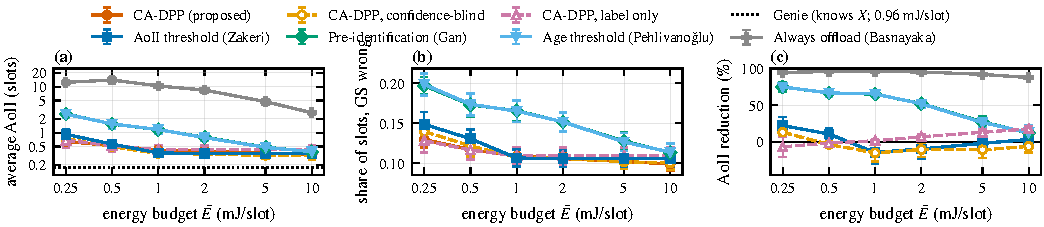
\includegraphics[width=\textwidth]{figures/fig_budget.pdf}
\caption{Energy budget sweep, $20$ held-out runs per point, with $95\%$ confidence intervals. (a) Average AoII. (b) Fraction of slots in which the GS is wrong. (c) AoII reduction by CA-DPP relative to each policy (paired intervals); negative values favor the other policy. Baselines are adapted from Zakeri et al.~\cite{zakeri2023aoiieh}, Gan et al.~\cite{gan2025taoi}, Pehlivano\u{g}lu et al.~\cite{pehlivanoglu2026orbit} and Basnayaka et al.~\cite{basnayaka2025aomi}.}
\label{fig:budget}
\end{figure*}

Fig.~\ref{fig:budget} and Table~\ref{tab:results} summarize the results. Against the pre-identification and age-threshold policies, CA-DPP lowers the AoII by $75\%$ at $0.25$\,mJ/slot, $52\%$ at $2$\,mJ/slot and $12\%$ at $10$\,mJ/slot, in every fold up to $5$\,mJ/slot ($p<10^{-5}$). The pre-identification policy spends most of its energy on labels that confirm what the GS already believes, which Proposition~\ref{prop:confirm} shows to be worthless. The age-threshold policy reacts to the time since the last delivery, which says little about whether the GS is wrong: an old status of a dry area that is still dry needs no update. Offloading every update is an order of magnitude worse at every budget, because a raw frame costs as much as $3$ to $21$ labels and fails often far from the GS.

Against the AoII-threshold policy, the outcome depends on the budget. At $0.25$\,mJ/slot, CA-DPP lowers the AoII by $22\%\pm12\%$ ($p=0.002$, four folds of five), and the $99$th percentile of the AoII drops from $19.2$ to $12.3$ slots. Here the UAV can send few labels, and the confidence decides which disagreements deserve them. At $0.5$\,mJ/slot the reduction is $11\%\pm7\%$ and not significant ($p=0.10$). From $1$\,mJ/slot on, the threshold policy with $k=1$ reports every disagreement for about $0.84$\,mJ/slot and matches CA-DPP; the differences range from $-3\%$ to $+14\%$ with $p\ge0.09$. When labels are this cheap, a wrong label is corrected by the next frame within a slot or two, which the one-step gain of Lemma~\ref{lem:onestep} ignores. We tested a discounted look-ahead over several slots of silence in place of the one-step gain, and it did not help.

\begin{figure}[t]
\centering
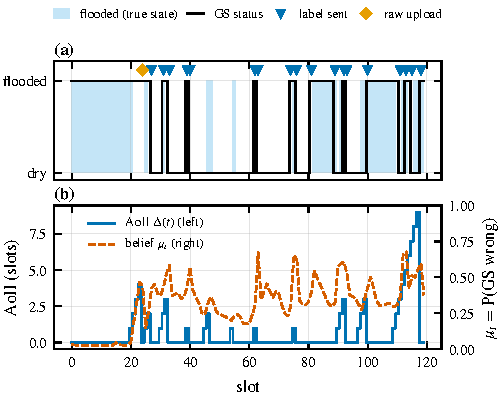
\includegraphics[width=\columnwidth]{figures/fig_path.pdf}
\caption{A sample path of CA-DPP at $\bar E=0.5$\,mJ/slot ($V=0.01$, $\nu=0.25$). (a) True state (shaded when flooded), GS status, and the slots in which the UAV sends a label (triangles) or uploads the frame (diamond). (b) AoII of the GS status (left axis) and the belief $\mu_t$ that the GS is wrong (right axis).}
\label{fig:path}
\end{figure}

Fig.~\ref{fig:path} shows CA-DPP over $120$ slots. The belief $\mu_t$ rises with each disagreeing frame; once it is high enough, the UAV sends a label and the AoII returns to zero. Over flooded stretches with patchy water, the classifier and the scene disagree often, and the UAV sends several labels in quick succession. A short AoII spike at the end of the window shows the cost of waiting: the belief rose more slowly than the true error, because the tempered update discounts the first disagreeing frames.

\subsection{Where the Gains Come From}
The ablations separate the contribution of the per-frame confidence from that of the raw uploads. At $0.25$\,mJ/slot the per-frame confidence matters: the confidence-blind version has a $15\%$ higher AoII ($p=0.001$). From $1$\,mJ/slot on, however, the confidence-blind version is $6\%$ to $15\%$ better than CA-DPP, and the difference is significant only at $1$\,mJ/slot ($p=0.02$). With this classifier, once energy is not scarce, the precision of each label value gives the belief most of what it needs. A plausible reason is the correlation of the on-board errors. A confident wrong label is often followed by another confident wrong label, and the per-frame update, even tempered, then raises the belief faster than it should. The per-label precision averages over such runs and is more robust to them.

Raw uploads pay off at larger budgets. Without them, the AoII stays at $0.43$ from $1$\,mJ/slot on, since the label-only version runs out of useful labels to send and spends only $0.65$\,mJ/slot. CA-DPP spends the rest of the budget on uploads and reaches $0.39$ at $2$\,mJ/slot and $0.34$ at $10$\,mJ/slot ($p\le0.001$). The genie reaches an AoII of $0.171$ with $0.96$\,mJ/slot. Most of the gap to it comes from not observing $X(t)$, which no policy can avoid.

\subsection{Weak Classifiers, Blockage and Payload}
\begin{figure*}[t]
\centering
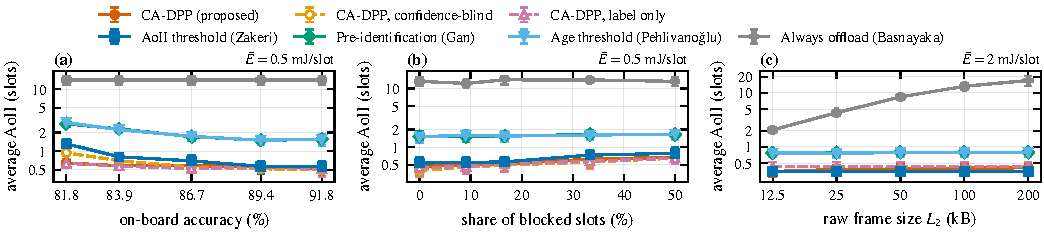
\includegraphics[width=\textwidth]{figures/fig_sensitivity.pdf}
\caption{Sensitivity, $20$ held-out runs per point. (a) On-board accuracy and (b) share of blocked slots, $\rho_{\rm b}/(\rho_{\rm b}+\rho_{\rm u})$, at $\bar E=0.5$\,mJ/slot. (c) Raw frame size at $\bar E=2$\,mJ/slot.}
\label{fig:sens}
\end{figure*}

Fig.~\ref{fig:sens}(a) lowers the on-board accuracy at $0.5$\,mJ/slot. The AoII of CA-DPP grows only from $0.53$ to $0.64$ as the accuracy drops from $91.8\%$ to $81.8\%$. Over the same range, the AoII of the threshold policy grows from $0.56$ to $1.31$, and that of the confidence-blind version from $0.50$ to $0.94$. At $86.7\%$ accuracy, CA-DPP is $12\%$ better than the threshold policy ($p=0.006$). With the two noisiest models, it is $27\%$ and $49\%$ better than the threshold policy ($p<10^{-5}$) and $14\%$ and $28\%$ better than the confidence-blind version ($p\le0.003$), in all five folds. With the two most accurate models the three policies are within the run-to-run spread. The noisiest model rarely says ``flooded'', so over a flooded area it mostly agrees with the wrong ``dry'' status of the GS. The threshold policy, which reacts only to disagreements, spends only $0.32$ of $0.5$\,mJ/slot. CA-DPP spends the full budget: a low-confidence ``dry'' frame barely lowers its belief that the GS is wrong, while a rare confident ``flooded'' frame raises it strongly, since flooded footprints are rare. The confidence-blind belief knows that ``dry'' labels are less reliable on average, but not which ones. Per-frame confidence therefore pays off when the classifier is weak and its errors are lopsided, as is likely for a small model on a low-cost device.

As the share of blocked slots grows from $0$ to $50\%$ (Fig.~\ref{fig:sens}(b)), all policies lose ground and their order is unchanged. CA-DPP stays $9\%$ to $15\%$ below the threshold policy ($0.009\le p\le0.1$). The confidence-blind and label-only versions are $1.5\%$ to $11\%$ below CA-DPP at this budget, so at $0.5$\,mJ/slot raw uploads cost slightly more than they return. Fig.~\ref{fig:sens}(c) varies the size of the raw frame at $2$\,mJ/slot. With $12.5$\,kB frames, CA-DPP is $15\%$ better than the label-only version and matches the threshold policy. With $200$\,kB frames the advantage over label-only shrinks to $3.5\%$, because uploads become more expensive and less reliable, and the policy uploads less often without any retuning.

\subsection{The Weight $V$ and the Role of Mobility}
\begin{figure}[t]
\centering
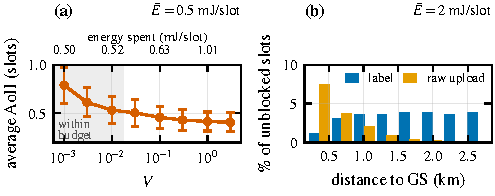
\includegraphics[width=\columnwidth]{figures/fig_V_mix.pdf}
\caption{(a) AoII of CA-DPP versus $V$ at $\bar E=0.5$\,mJ/slot; the top axis gives the energy spent, and the shaded values of $V$ stay within $4\%$ of the budget. (b) Share of unblocked slots with a label or a raw upload versus the distance to the GS, at $\bar E=2$\,mJ/slot.}
\label{fig:Vmix}
\end{figure}

Fig.~\ref{fig:Vmix}(a) shows the trade-off governed by $V$ at $0.5$\,mJ/slot. Raising $V$ from $10^{-3}$ to $3$ lowers the AoII from $0.79$ to $0.41$. A larger $V$, however, lets the energy debt grow larger before it raises the price, and over a run of about $27{,}000$ slots the energy spent rises from $0.50$ to $1.51$\,mJ/slot. Values of $V$ up to $10^{-2}$ stay within $4\%$ of the budget. This is the finite-horizon face of Theorem~\ref{thm:budget}: the budget is met in the long run for every $V$, but the transient excess grows with $V$, so $V$ must be matched to the mission length.

Fig.~\ref{fig:Vmix}(b) shows how CA-DPP exploits the trajectory at $2$\,mJ/slot. Within $850$\,m of the GS, where uploads are cheap and reliable, it uploads the frame in $5.9\%$ of the unblocked slots and sends labels in $2.0\%$. Beyond $2.15$\,km it uploads in only $0.1\%$ and sends labels in $3.8\%$. The UAV thus asks the ground when asking is cheap and relies on its own labels when it is not, with no rule that refers to the distance explicitly. The distance enters only through $q_a(g)$ and $E_a(g)$ in~\eqref{eq:rule}.

%% =====================================================================
\section{Discussion}\label{sec:discussion}
%% =====================================================================
\subsection{When Does the Confidence Pay Off?}
The per-frame confidence helps when updates are scarce, either because energy is scarce or because the classifier is weak. In both cases the UAV must choose which few disagreements to report, and the confidence ranks them. When energy is ample and the classifier is accurate, the UAV can report every disagreement, a wrong label is corrected within a slot or two, and a simple rule does as well as the belief. Three lessons for the design of IoT devices with on-board inference follow.

First, a device should never send a label that agrees with the receiver (Proposition~\ref{prop:confirm}). This rule alone separates the AoII-threshold policy and CA-DPP from the pre-identification and age-threshold policies, which differ from them by $52\%$ to $75\%$ at moderate budgets.

Second, the classifier should be calibrated on board. Isotonic calibration is a lookup table at run time, and it lets the belief use the confidence as a probability. The prior correction~\eqref{eq:lik} matters for unbalanced classes, which are the rule in monitoring: floods, fires and intruders are rare.

Third, the value of raw uploads depends on the link more than on the classifier. Uploads paid off at budgets of $2$\,mJ/slot and above, near the GS, and with small frames. At tight budgets the UAV almost never uploads, and the label-only version performs as well as the full policy.

\subsection{Correlated Errors}
The main weakness of CA-DPP at large budgets is Assumption~\ref{as:inf}(ii). The on-board errors in our traces come in runs (Fig.~\ref{fig:inference}(c)): an error is followed by another error with probability $0.56$, against a marginal error rate of $0.08$. The tempered update~\eqref{eq:post} discounts every frame equally, which helps on average but does not distinguish a new piece of evidence from a repetition of the last one. A belief that models the error process explicitly, for example with a hidden Markov model of the classifier state, could do so. It would enlarge the belief by a factor of two and change Step 1, but Lemma~\ref{lem:onestep} would still apply, since it depends only on $\mu_t$ and $S_t$. We see this as the most promising way to improve the policy at large budgets.

\subsection{Other IoT Settings}
Nothing in the model is specific to UAVs or floods. The link model~\eqref{eq:succ} and the energy model~\eqref{eq:energy} apply to any device whose channel varies predictably, such as a satellite in low Earth orbit that sees a ground station only during passes, or a ground sensor that wakes up on a schedule. For a satellite, long outages are predictable, and a version that spends more just before an outage, through the renewal formulation of Remark~\ref{rem:opt}, would anticipate them. A non-binary scene, such as a land-cover class, requires a belief over the AoII and the current class, but the structure of the gains carries over: an update removes AoII when the GS is wrong and the update right, and creates AoII in the opposite case.

\subsection{Limitations}
Five limitations remain. First, the policy minimizes the AoII of the next slot only, and we have no bound on its gap to the optimal policy of (P). Second, the threshold structure of Proposition~\ref{prop:threshold} is proved for the per-slot rule~\eqref{eq:rule} with a constant ground error. Whether the optimal policy of (P) has the same structure is open. Third, the Sentinel-2 imagery is a proxy for UAV frames. UAV frames have higher resolution, a different viewing geometry and motion blur, which would change both classifiers. Repeating the study with UAV datasets such as FLAME~\cite{shamsoshoara2021flame} and AIDER~\cite{kyrkou2020aider} is the next step. Fourth, the energy model is analytic. Measuring the energy of inference and transmission on a microcontroller would test whether the label really costs a tenth of an upload in practice. Fifth, the photo sequence and the UAV position are generated separately, so the imagery is not tied to the location on the circle. A spatial model of the area, with correlated neighboring patches, revisits and a route chosen by the UAV, is left for future work.

%% =====================================================================
\section{Conclusion}\label{sec:concl}
%% =====================================================================
We studied status updates from an IoT device whose sensor is its own classifier, with a UAV mapping a flood as the running example. The device tracks a belief over the AoII of the ground station's status, updated with the calibrated confidence of each frame. The belief gives closed-form one-step values of the three actions, which show that agreeing labels are worthless and that the per-slot decision has confidence thresholds ordered silent, raw, label. The online policy CA-DPP built on them meets the energy budget on every sample path and keeps a belief of about 1.2\,kB. On flood-mapping traces under chip-level cross-validation, it outperforms adaptations of three recent designs at every budget up to $5$\,mJ per slot. Against an AoII-threshold policy it helps when energy is scarce or the on-board classifier is weak, because then the confidence decides which disagreements are worth reporting. With an accurate classifier and ample energy, reporting every disagreement works as well. A belief that models the correlation of on-board errors, a performance bound through the renewal framework, experiments with UAV imagery and measured energy, and a spatial model of the area are the next steps.


\appendices
\section{Proof of Lemma~\ref{lem:mono}}\label{app:mono}
Let $y=\Lambda_t^{\nu}$, which increases with $\Lambda_t$. By~\eqref{eq:post}, the mass at every $\delta>0$ is multiplied by $y/D$ and the mass at $\delta=0$ by $1/D$, with $D=1-\mu^-_t+\mu^-_ty$. Hence
\[
S_t=\frac{y\,S^-_t}{D},\qquad 1-\mu_t=\frac{1-\mu^-_t}{D},
\]
and $AS_t-B(1-\mu_t)=N/D$ with $N=AyS^-_t-B(1-\mu^-_t)$. Both $N$ and $D$ are affine in $y$, so the derivative of $N/D$ with respect to $y$ has the sign of
\begin{multline*}
AS^-_t\big(1-\mu^-_t+\mu^-_ty\big)-\big(AyS^-_t-B(1-\mu^-_t)\big)\mu^-_t\\
=(1-\mu^-_t)\big(AS^-_t+B\mu^-_t\big)\ \ge\ 0.
\end{multline*}
Since $D>0$, $N/D$ is nondecreasing in $y$, and hence in $\Lambda_t$. \hfill$\blacksquare$

\section{Proof of Proposition~\ref{prop:threshold}}\label{app:threshold}
Let $f_a=Vq_aG_a-\lambda E_a$ be the objective of~\eqref{eq:rule}, so $f_0=0$. Since $r,w<\frac12$ and $\ee_{\rm g}\le1$, both gains have the form $AS_t-B(1-\mu_t)$ with $A,B\ge0$: for $G_2$, $A=(1-\ee_{\rm g})(1-2w)$ and $B=\ee_{\rm g}(1-2r)$, and for $G_1$ with $d(t)=1$, $A=1-2w$ and $B=1-2r$. The difference $q_1G_1-q_2G_2$ has the same form, with
\[
A=(1-2w)\big(q_1-q_2(1-\ee_{\rm g})\big),\qquad B=(1-2r)\big(q_1-q_2\ee_{\rm g}\big),
\]
both nonnegative because $q_2\le q_1$. By Lemma~\ref{lem:mono}, $f_2-f_0=Vq_2G_2-\lambda E_2$ and $f_1-f_2=V(q_1G_1-q_2G_2)-\lambda(E_1-E_2)$ are nondecreasing in $\Lambda_t$, and so is their sum $f_1-f_0$.

(a) If $d(t)=1$, then $\Lambda_t$ increases in $c$. Order the actions as $0\prec2\prec1$. The differences between consecutive actions in this order are nondecreasing in $c$, so $f_a$ has increasing differences in $(a,c)$. By Topkis' theorem, the largest maximizer of $f_a$ is nondecreasing in $c$ in this order; with ties broken toward silence, the same holds for the selection of Algorithm~\ref{alg:dpp}. Hence the action moves from 0 to 2 to 1 as $c$ grows, which defines $c_{\rm r}\le c_{\lab}$.

(b) If $d(t)=0$, then $G_1=0$ by Proposition~\ref{prop:confirm}, so $f_1=-\lambda E_1\le f_0$ and the label is never strictly preferred to silence. Now $\Lambda_t$ decreases in $c$, so $f_2-f_0$ is nonincreasing in $c$, and the set of $c$ for which $f_2>f_0$ is an interval of the form $\{c\le c^0_{\rm r}\}$.

(c) For fixed $\mu^-_t$ and $\Lambda_t$, $S^-_t$ appears in $N/D$ only in the numerator, with coefficient $Ay\ge0$. So $f_a-f_0$ is nondecreasing in $S^-_t$ for $a\in\{1,2\}$, and a slot in which some action beats silence still has one when $S^-_t$ grows. Each $f_a-f_0$ with $a\neq0$ decreases in $\lambda$, so a slot in which silence is optimal remains so when $\lambda$ grows. \hfill$\blacksquare$

\section{Proof of Theorem~\ref{thm:budget}}\label{app:budget}
We first bound the gains. Since the belief is truncated at $\Delta_{\max}$, $S_t=\E_{\pi_t}[(\Delta+1)\ind{\Delta>0}]\le\Delta_{\max}+1$. By~\eqref{eq:G1} and~\eqref{eq:G2}, $G_a\le S_t$ for $a\in\{1,2\}$, because the negative terms can be dropped and $(1-2w)(1-\ee_{\rm g})\le1$. With $q_a\le1$, $Vq_aG_a\le V(\Delta_{\max}+1)$.

Let $z^\star=V(\Delta_{\max}+1)/E_{\min}$. If $Z(t)>z^\star$, then for $a\in\{1,2\}$,
\[
Vq_aG_a-Z(t)E_a(g)<V(\Delta_{\max}+1)-z^\star E_{\min}=0=f_0,
\]
so CA-DPP stays silent, and~\eqref{eq:Z} gives $Z(t+1)=\max\{Z(t)-\bar E,0\}\le Z(t)$. If $Z(t)\le z^\star$, then $Z(t+1)\le Z(t)+E_{\max}\le z^\star+E_{\max}$. Starting from $Z(0)=0$, induction on $t$ gives $Z(t)\le z^\star+E_{\max}=Z_{\max}$ for all $t$. Inserting this bound in~\eqref{eq:Zbound} gives the energy bound for every $T$, and taking expectations and $T\to\infty$ gives~\eqref{eq:budget}. \hfill$\blacksquare$


\bibliographystyle{IEEEtran}
\bibliography{refs}

\end{document}
